\documentclass[journal]{IEEEtran}

\usepackage{palatino,epsfig,latexsym,cite,graphicx,amsmath,amssymb,amsfonts,multirow,booktabs,color,soul}
\usepackage{algorithmic,url}
\usepackage{float}
\usepackage{paralist}
\usepackage{threeparttable}
\usepackage{amsmath}
\usepackage[linesnumbered,ruled,vlined]{algorithm2e}
\def\MR2{\multirow{2}[2]{*}}
\def\Hei{\hl}
\definecolor{hl}{rgb}{0.75,0.75,0.75}
\newcommand{\XG}[1]{\textcolor[rgb]{0.00,0.00,1.00}{#1}}
\newcommand{\TODO}[1]{\textcolor[rgb]{1.00,0.40,0.22}{#1}}
\sethlcolor{hl}
\usepackage{makecell}
% \usepackage{subfigure}
\usepackage[caption=false,font=footnotesize]{subfig}
\renewcommand{\algorithmicrequire}{ \textbf{Input:}}      %Use Input in the format of Algorithm
\renewcommand{\algorithmicensure}{ \textbf{Output:}}     %Use Output in the format of Algorithm
\DeclareMathOperator*{\argmin}{argmin}
\DeclareMathOperator*{\argmax}{argmax}

%\setlength{\abovecaptionskip}{-5pt}
\setlength{\floatsep}{12pt  minus 4pt}
\setlength{\textfloatsep}{13pt minus 4pt}
\renewcommand{\textfraction}{0.1}
\renewcommand{\topfraction}{0.9}
\setlength\arraycolsep{2pt}

\begin{document}

\title{{Adaptation Operator Selection with Reinforcement Learning for Multi-objective Evolution}
  \thanks{Thanks}}
\author{
  authors,
}% <-this % stops a space

% \markboth{IEEE Transactions on Cybernetics,~Vol.~, No.~, month~year}
% {Tian \MakeLowercase{\textit{et al.}}: SOLVING LMOPS WITH SPARSE OPTIMAL SOLUTIONS VIA UNSUPERVISED NNS}

\IEEEpubid{0000--0000/00\$00.00~\copyright~0000 IEEE}

\maketitle

\begin{abstract}
  % 进化算法是一种受算子影响较大的随机优化算法,不同的复制算子具有不同的搜索范围。
  Evolutionary Algorithms (EAs) are stochastic optimization algorithms which are greatly influenced by operators, different operators have various search ranges.
  % AOS提供对进化算法的在线控制,即为当前个体选择合适的算子。
  Adaptive operator selection (AOS) provides the online control of the evolutionary algorithms that is, to choose the appropriate operator for the current individual.
  % 本文提出了一种基于DQN的算子选择策略,来确定哪个算子将被应用
  This paper proposed a new AOS approach based on Deep Q Network (MOEA/D-DQN), a Deep Reinforcement Learning (RL) algorithm in discrete action spaces, to determine which operator will be applied.
  % AOS的两部分信誉赋值和算子选择,分别对应MDP中的reward和action,当前个体的特征可以作为MDP的state,
  The two main components of AOS, \textit{Credit Assignment} and \textit{Operator Selection}. The first defines how to reward an operator based on its recent applications, while the second uses rewards to decide which operator should be selected.
  %  and the state of MDP can be represented by the features of the current individual.
  % 算子选择问题通常被建模为MAB问题,并用RL解决
  Adaptive operator selection problem is usually modeled as Multi-armed Bandit (MAB) problem and can be solved by reinforcement learning.
  % 在进化过程中,
  In the evolutionary process, RL will select an operator for each individual and update the behavioral strategy according to the effect of this selection.
  Experimental results show that our proposed MOEA/D-DQN performs better than the other two adaptive operator selection methods (MOEA/D-FRRMAB and MOEA/D-DYTS), and has better performance than other MOEA/D variants (MOEA/D-DRA and MOEA/D-M2M).
\end{abstract}

\begin{IEEEkeywords}
  Multi-objective optimization, Reinforcement Learning, Adaptive operator selection
\end{IEEEkeywords}

\section{Introduction}
%%%%%%%%%%%%%%%%%      需要在introduction里说明我的算法,包括主要的过程,实验部分,和其它RL的相关知识

%%% 介绍下进化多目标优化
% 由于多个目标间通常互相冲突,没有一个全局最优解,一般会有一个PF
\IEEEPARstart{M}{ultl-object} optimization problems (MOPs) are characterized by multiple objectives that often conflict with each other\cite{zhang2014efficient}. In general, MOPs have no single optimal solution on all objectives; instead, a number of solutions are optimal for different objectives, known as Pareto-optimal solutions.
% All the Pareto optimal solutions constitute the Pareto set and the set of all Pareto optimal objective vectors is the Pareto front \cite{deb2001multi}.

%%%%%%%%%%%%% 介绍进化算法
% 进化算法可以解决很多多目标优化问题,最近几十年有了很大的发展,
Multi-object evolutionary algorithms (MOEAs) have attracted extensive attention over the past few decades and achieved outstanding performance in solving various kinds of MOPs \cite{fialho2010adaptive},
% 人们提出了很多新的算法,主要有3类,基于支配关系的,基于分解的和基于指标的算法
many algorithms have been proposed, e.g., indicator-based evolutionary algorithm (IBEA) \cite{IBEA}, the multi-objective evolutionary algorithm based on decomposition (MOEA/D) \cite{moead} and fast non-dominated sorting genetic algorithm (NSGA-II) \cite{nsga2}.
% 生成算子对进化算法的性能有很大的影响,有的算子注重探索能力,我们称为全局算子,有的注重局部的收敛,我们称为局部算子,那么如何平衡算法的探索和利用就成了人们研究的对象
In these algorithms, the reproduction operators have a great influence on the performance.
Generally speaking, different operators have different applications, some operators tend to explore unknown regions to find global optimal solutions, called global operators; and the others tend to converge quickly with population information, called local operators.
% 所以我们要平衡探索和利用算子
In order to accelerate the process of evolution, balanced exploration and exploitation became an important topic.

%%% 介绍AOS
% 在进化算法中,有多个变异策略可以用来从父代产生子代解
In evolutionary algorithms, multiple operators can be applied at each generation to produce new solutions from parent solutions.
% AOS是确定应用哪个算子的方法,衡量应用的效果,并且更新算子的credit并且adapt选择策略
AOS is an approach that decides which operator should be applied, measure the effect of this application, update the credit of operators and adapt the selection strategy \cite{li2011multi}.
% AOS就是为个体推荐合适的算子,在线控制
% Adaptive operator selection (AOS) applies appropriate operators for individuals by online control while solving the problem, based on the recent performance of operators \cite{li2011multi}.
% 包含credit assignment和operator selection 两部分,
An AOS algorithm usually consists two components: \textit{credit assignment} and \textit{operator selection}. Credit assignment rewards an operator based on its recent performances in the search process and the operator selection determines which operator should be selected according to their rewards.
% 和credit assignment 尽量准确评价算子近期的效果不同,operator selection 需要平衡探索和利用,即既需要选择尽量表现好的算子来提高算法效果,又需要给表现不好的算子一些机会,因为它们在之后有可能变好。
Different from credit assignment, which only needs to evaluate operator performance as accurately as possible, operator selection should balance exploration and exploitation: one hopes to give more chances to the best operators found so far in order to maximize the cumulative improvement (exploitation), but also needs to explore poor operators in the future search (exploration).
% 通常有MAB,UCB,可以和MOEAD结合应用到多目标问题上。
% 但是由于环境是不稳定的,一开始好的算子不一定在最后好,所以就有动态MAB或者动态汤普森采样等。
% 写到related work里吧

%%%%%%% 介绍RL
% 根据状态做出动作的强化学习正适合用来解决探索和利用困境
Reinforcement Learning (RL) that selects actions according to the state is good at solving Exploration vs. Exploitation dilemma.
% 介绍强化学习
An RL agent interacts with its environment in discrete time steps, at each time $t$, the agent receives the current state $s_t$ and reward $r_t$. It then chooses an action $a_t$ from the set of available actions, which is subsequently sent to the environment. The environment moves to a new state $s_{t+1}$ and the reward $r_{t+1}$ associated with the transition $(s_t, a_t, s_{t+1})$ is determined. The goal of a reinforcement learning agent is to learn a policy $\pi(a, s)=\operatorname{Pr}\left(a_{t}=a \mid s_{t}=s\right)$ which maximizes the expected cumulative reward.

%%%%%%%%% 将RL应用到AOS
% 在自适应算子选择问题中,我们可以将多目标优化问题和当前的种群作为环境,将选择算子作为动作,应用所选算子后环境负责给出下一个状态并且评价动作的reward,
In the AOS problems, we take MOPs and the current population as environment, take the selection operator as action, after application of the operator, the environment will give the next state and evaluate the reward of the action.
% 将算子作为动作,将应用算子后种群发生的变化作为奖励,
% In the AOS problems, we take MOPs and the current population as environment, take the population characteristics as states, take the operators as actions and the improvement of population fitness after the application of the operator is regarded as the reward.
% 我们会发现遗传算法和强化学习在概念和结构上有相似性
Viewed in this light, GA can be regarded as similar to RL in its evolution/learning structure, which causes high conceptual and structural compatibility between RL and GA.

%%% 介绍本文
% 现有的AOS方法,比如moead-frrmab和FAME,根据算子近期的表现选择算子,当算法运行到不同阶段时,会及时替换算子以满足问题的需要,
Existing AOS methods, such as MOEA/D-FRRMAB \cite{frrmab} and FAME \cite{fame}, select an operator from the recent operator performances when the algorithm runs to different states, it will replace the operator in time to meet the needs of the problem.
% 但是即使在同一阶段,针对不同的个体,不同的子问题,最佳的算子也是不同的,因此算子选择策略不应该只考虑阶段性的差异,也应该考虑不同个体间的差异
Even at the same state, the best operator is different for different individuals and different subproblems. \XG{ Therefore, the AOS strategy should not only consider the differences of stages, but also consider the individual differences.}
% 本文提出了一种基于RL的AOS方法,该方法可以根据个体推荐不同的算子来实现更细粒度的控制,并分别推荐交叉算子和变异算子来达到更好的控制效果
In this paper, we proposed an AOS method based on RL, which can recommend different operators according to the individual to achieve more fine-grained control and recommend crossover operators and mutation operators respectively to achieve better results.

% 本文组织结构
% 在第二章,我们介绍了多目标优化,强化学习的和AOS的相关工作. 在第三章,我们提出了MOEA/D-DQN,并详细介绍了实现细节。实验结果
The rest of this paper is organized as follows. In Section II, we introduced the background of AOS and some related works. We proposed AOS methods MOEA/D-DQN and introduced the details of its implementation in Section III. In Section IV, the experimental results are presented and analyzed. At last, we give the main conclusions and lines for future research in Section V.

\IEEEpubidadjcol

\section{Background and Related Work}
%%% 进化算法的效果和产生子代的策略有关,为了充分利用不同算子,最近几年提出了很多自适应算子选择的策略。
The performance of EAs mainly depends on its generating Offspring strategy, to take full advantage of several effective operators, many adaptive operator selection strategies have been proposed in recent years.
% 这一章节介绍AOS用到的概念和背景知识,和一些相关的工作。
This section provides some basic concepts, background knowledge, and some related work about AOS.

\subsection{Multi-objective Optimization}
%%% 介绍多目标优化和MOEAD
Multi-objective optimization problems are usually formulated as follows:

\begin{equation}
  \begin{array}{ll}
    \text { Minimize: }   & \mathrm{f}=\left\{f_{1}(\mathrm{x}), \ldots, f_{M}(\mathrm{x})\right\} \\
    \text { Subject to: } & l_{d} \leq x_{d} \leq u_{d} \quad d=1, \ldots, D
  \end{array}
  \label{eq: moea}
\end{equation}

%============ 介绍多目标优化
% x是决策变量,f是一组互相冲突的目标函数,由于目标是冲突的,所以不存在一个解可以在所有目标上达到最优,
Where $x = (x_1, \cdots ,x_D)$ is a decision variable vector of length $D$, $l$ and $u$ are the lower and upper bounds of the decision variables. $f$ consists of $M$ conflicting objective functions. Since the objectives are conflicting, there is no one solution that is optimal for all objectives.
% 所有可能的解构成决策空间,决策空间可以由目标函数对应到目标空间,在目标空间中,如果一个解在所有目标上都不比另一个差,且至少在一个目标上比另一个好,我们就称为一个解支配另一个解。
All possible decision variables constitute the decision space and objective functions can be mapped from the objective space to the decision space\cite{gonccalves2017adaptive}. In the objective space, one solution is said to dominate the other solution if it is no worse than the other solution on all objectives and is better than the other solution on at least one objective.
% 当一个解不被支配时就是Pareto最优解
A solution $x^*$ is said to be Pareto-optimal when no other solution can dominate $x^*$. All the Pareto-optimal solutions constitute the Pareto set, and the image of the Pareto set in objective space is called the Pareto front \cite{deb2001multi}.

%=========== 主要框架是MOEA/D,所以肯定要大略介绍下
% 将AOS应用到多目标上的工作很少,因为多目标很难定量的描述子代相对于父代适应度的提高,
Very little work has been done to apply AOS to multi-objective evolutionary algorithms since it is difficult to measure the increase in fitness of the offspring relative to the parent.
% 
% 在论文中,我们使用MOEA/D作为主要的多目标优化框架,MOEAD的基本思想是将多目标问题分解成多个单目标的子问题,将AOS与MOEA/D结合是合适的,因为单目标的AOS方法可以transfer to MOEAD
In this paper, we use MOEA/D-DRA \cite{moead-dra} as the evolutionary multi-objective optimization framework. The basic idea of MOEA/D-DRA is to decompose a multi-objective optimization problem into several scalar optimization subproblems and optimizes them together.
It is appropriate to combine AOS with MOEA/D-DRA because the single objective AOS method can be easily transferred to MOEA/D-DRA.

% 在传统的MOEA中,算法的性能取决于变异算子的质量。一个好的变异算子可以大大提高算法的搜索能力,从而获得更好的收敛和收敛速度。
The performance of MOEAs is closely related to the quality of operators, a high quality operator can greatly improve the searchability of the algorithm, to obtain better convergence and convergence speed.
% 在过去的二十年里,人们提出了许多非常好的算子,包括经典的突变算子 模拟二进制交叉(SBX)[6]和差分进化(DE)[15]SBX操作符在本地搜索中表现更好,而DE操作符以其强大的全局搜索能力而闻名,
In the past two decades, many excellent operators have been proposed, including the Simulated Binary Crossover \cite{deb2006reference} and Differential Evolution \cite{storn1997differential}, The SBX operator is good at local search and the DE operator is famous for its powerful global searchability.
% 然而,不同的实验向量生产策略和参数选择对moea的性能有很大的影响,通常没有一个单独的算子可以在所有问题上都表现良好。
However, different experimental vector selection strategies and parameter settings have a great impact on the performance of MOEA, generally, there is no single operator that can perform well on all problems.
% 所以我们需要针对不同的问题选择不同的算子和参数, 然而,在现实生活中,问题是事先未知的。因此,当一个复杂的MOP出现时,为其选择参数是困难的
So we need to select operators and parameters for different problems. However, in real-world, the problem is unknown in advance. Therefore, when a complex MOP appears, it is difficult to select an operator to solve the problem.

\subsection{Adaptive Operator Selection}
%%% 介绍自适应算子选择
% 自适应算子选择是控制变异算子在线应用的一种方,选择的依据是算子在之前的表现.法
AOS is an approach for controlling online the application of the variation operators \cite{hitomi2016classification}, the selection is based on the previous performance of the operator.
% --- TODO: 介绍MOEAD与AOS结合后的处理流程
% AOS主要有两个任务,适应度赋值(评价算子)和算子选择(依据评价做出选择)。
%%%%%%%%%%%%%%%%%% 补充图片,介绍适应度赋值和算子选择的联系
AOS requires two tasks to be solved, the \textit{Credit Assignment} strategy that defines how to evaluate an operator based on its performance in the search process and the \textit{Operator Selection} strategy that determines the next operator according to the quality of the operator.

\subsubsection{Credit Assignment}
%%%%%%%%%%% 信誉分配
% 信誉赋值定义如何基于算子最近的应用带来的影响评估算子的质量
Credit assignment defines how to estimate the quality of operators based on the impact of their recent applications.
% 最常用的信誉分配方法是根据子代相对于父代的适应度提高来确定
The most common method of credit assignment rewards an operator for its performance to improve the fitness of an offspring over its parent, in \cite{lin2016adaptive} the fitness improvement rates (FIR) is obtained with the used operator
, as defined in Equation (\ref{eq:fir}),

\begin{equation}
  \text{FIR}_{i}=\left\{
  \begin{array}{ll}
    \frac{pf_{i}-cf_{i}}{pf_{i}} & \text{if }pf_{i}-cf_{i}>0 \\

    0                            & \text{otherwise}
  \end{array}
  \right.
  \label{eq:fir}
\end{equation}

% pf和cf分别是父代和子代的适应度值,如果父代比子代差,子代不会插入到父代中,因此FIR=0
where $pf_{i}$ and $cf_{i}$ are the fitness values of the parent and its offspring, if the offspring is worse than the parent, then set FIR to 0.
% 由于有写目标函数值的量级不同,如果我们知道真实最优值,一般用父代与真实最优值的差做分母。
In order to track the dynamics of the search process, ExAOS \cite{fialho2008extreme} use a sliding window to save recent fitness improvement rates produced by the operators,
% 有观点认为稀少但巨大的改进比频繁但微小的改进更有用
some people believe the operators that make rare but large improvements are more important than operators that make frequent and small improvements \cite{fialho2009dynamic},
% 滑动窗口里存提高率,reward是滑动窗口里operator对应的最大值,
the operator reward is set to the maximal fitness improvement in the time windows, credit assignment strategy rewards the operators that generate a high quality of offspring.
% 除了上面的奖励方法,还有文章根据分布性奖励算子
In addition there are some strategies reward operators that increase the fitness of the solution while maintaining the diversity of the solution set \cite{auer2002finite}.

% 大多数的AOS研究都是关于单目标的,因为多目标很难做信誉赋值,而且也不容易比较解
Most of the studies on credit assignment in AOS are for single-objective problems, such as \cite{fialho2009dynamic,cowling2000hyperheuristic}, and there has been little work done on AOS in multi-objective evolutionary computation because it is very difficult to define the credit assignment and compare one solution to another.

% 现有的多目标信誉赋值在比较个体和赋值方式上有所不同
The existing multi-objective credit assignment is different in which individuals should be compared and assigning strategies, most of the AOS for MOPs is based on differential evolution.
% 有些工作是基于支配关系的,
Some previous works reward operators based on the dominant relationships,
% MOSaDE依据帕累托支配关系和拥挤距离来奖励算子。
such as MOSaDE \cite{huang2007multi} rewards an operator if it is better than incumbent solution in terms of Pareto-dominance and crowding distance.
In MCHH \cite{mcclymont2011markov}, the reward of an operator is determined by the offspring it produces that dominate many solutions from the previous generation. Adap-MODE \cite{li2011multi} rewards an operator according to the fitness improvement of a solution, where fitness is the weighted sum of Pareto metric and density metric.
% 有一些基于支配关系奖励算子的工作。比如在AMALGAM中,
% 最近的一些工作大多是基于分解的多目标算法,比如FRRMAB,根据基于分解的适应值函数评价算子对于目标函数值的提高能力
Most of the recent works are based on decomposition of the multi-objective algorithm, such as MOEA/D-FRRMAB \cite{frrmab}, which reward an operator according to its improvement of decomposition-based fitness value compared with the neighboring subproblems.
% B-AOS 双标准的辅助的AOS,一个指标是收敛性,另一个指标是分布性。
B-AOS \cite{lin2021decomposition} proposed a bicriteria-assisted adaptive operator selection strategy, in which one criterion reflecting the convergence according to the Pareto dominant relation and another criterion reflecting the diversity according to the crowding distance.
% 算法在前期比较注重分布性,在后期更加注重收敛性。
The algorithm keeps the distribution of the population in the early stage and pays more attention to the convergence of the population in the later stage.
% 也有一些基于支配关系的工作,
On the other hand, AMALGAM \cite{vrugt2007improved} rewards the operator according to the number of solutions it contributes to the population.
% 通常来讲,有三种基于支配关系的奖励方式。
Generally speaking, there are three different credit assignments based on dominance, offspring-dominates-parent (ODP), Pareto front (PF), and Pareto rank (PR) \cite{hitomi2015effect}.

\subsubsection{Operator Selection}
% 和信誉赋值相比,
% Compared with credit assignment, the operator selection 
% 信誉赋值之后就可以根据算子的信誉为个体推荐合适的算子,但不能直接选择credit最高的算子,因为这会使我们丢失多样性
After credit assignment, we can recommend appropriate operators for individuals according to the credit of operators, but we can not choose the operator with the highest credit directly, because it will make population lose diversity.
% 一方面,我们需要给好的算子更多机会,另一方面我们需要探索较差的算子,因为它们可能在未来表现出显著的不同,我们称之为探索利用困境。
On the one hand, we need to give more opportunities to operators with better track records, on the other hand, we need to explore poor operators, since an operator might perform significantly differently in the future search stages, we called this difficult as exploration versus exploitation (EvE) dilemma.

%%% 和前面credit assignment类似的介绍不同工作的算子选择方案,
% DMAB和SLMAB

%  ExAOS

%  MOSaDE

% MCHH

% Adap-MODE

% MOEA/D-FRRMAB

% B-AOS

% AMALGAM





% 一个常用的方法是概率匹配算法
A common method is probability matching (PM) algorithm \cite{thierens2007adaptive}, each operator $o_i$ in the operator pool $O$ has a corresponding probability value $p_{i,t}$ as generation $t$, $p$ is determined by the quality $q_{i,t}$, $q$ is updated according to the reward $r_{i,t}$ received during the credit assignment phase, and the formula is as follows:
\begin{equation}
  q_{i,t+1} = q_{i,t} + \alpha(r_{i,t} - q_{i,t})
  \label{eq: pm_q}
\end{equation}
% 这是利用时序差分法,根据算法的reward估计算子的质量。
with the learning rate $\alpha \in (0,1]$, using the Temporal-Different method to estimate the quality of operator.
% 然而,如果有算子在当前的概率=0,那么他在之后就永远不会被选中,quality也不会被更新
Once a quality $a_{i,t}$ becomes equal to 0, the operator will never be selected in the future and its quality can no longer be updated.
% 在非平稳的环境中,该算子可能在之后会有更好的表现,所以
In a non-stationary environment, the operator might perform better in a future stage of the search process.
% 为了避免有的算子概率太小以至于长时间不被 measure  the  improvement  of  offspring选择,PM设定一个最小选择概率称为 Pmin,
So in order to avoid the operator probability is too small to be selected, PM designs a minimal probability, $p_{min}: 1 > p_{min} > 0$, for exploring currently underperforming operator. Since the total probability is 1, thus we can get the update rule of $p_{i,t}$:
\begin{equation}
  p_{i,t+1} = p_{min} + (1-k \cdot p_{min}) \frac{q_{i,t+1}}{\sum_{i=1}^k q_{i,t+1}}
  \label{eq: pm_p}
\end{equation}
Where $k$ is the number of operators.
% PM在很多差算子的情况下很难获得好的结果, 因为多个差的算子的和也是很大的。
When there are many mediocre operators and only one efficient operator, it is difficult for the PM algorithm to achieve high performance, because the minimal selection probability for each operator is $p_{min}$, the sum of selection probabilities from many mediocre operators has a significant advantage over the high-performance operator.

% 引入AP方法,赢家通吃的策略,提高最佳算子被选中的概率,降低其它算子的概率。
Another method based on probability is Adaptive Pursuit (AP) \cite{thierens2007adaptive}, which adopts the winner-take-all strategy to allocate the best operator with higher probability, the pursuit method increases the probability of the best operator $a^*$ being selected and reduces the probabilities of other operators.
% AP的过程介绍,根据Pmin算出Pmax
Like PM, AP also designs the minimum probability $p_{min}$, while an operator that works well can obtain the maximum selection probability $p_{max} = 1-(k-1)\times p_{min}$.
% AP 追踪当前最佳的算子o^*,
AP pursues the best operator $o^*$ with the maximal quality, to avoid the disadvantages of PM, AP increases the selection probability of the best operator $p_{o^*,t}$ and decreases the other probabilities $p_{o,t}, \forall o \neq o^*$ by the following formula.
\begin{equation}
  p_{i, t+1}=\left\{\begin{array}{ll}
    p_{i, t}+\beta \cdot\left(p_{\max }-p_{o, t}\right) & \text { if } o=o^{*} \\
    p_{i, t}+\beta \cdot\left(p_{\min }-p_{o, t}\right) & \text { otherwise }
  \end{array}\right.
  \label{eq: AP}
\end{equation}
Where $\beta \in (0,1]$ is the learning rate.
% 
% 搜索过程中,算子的性能可能是动态变化的,因此在算子选择中最困难的就是平衡探索和利用。
% The performance of operators may be dynamic in the search process, so the most difficult problem in operator selection is to balance exploration and exploitation.
% 
% 由于进化过程是动态的,算子的性能在不同阶段可能有很大的差异,AP和PM可能没有办法适应剧烈变化的环境
Due to the dynamic nature of the evolution process, an operator might perform significantly differently in different stages, when credit changes rapidly, PM and AP may not be able to quickly adjust their selection strategies.

% 在多臂赌博机的框架下 EvE困境已经被深入研究
In the Multi-Armed Bandit (MAB) framework, the EvE trade-off has been intensively studied.
% 原始的MAB框架使用UCB的方法, 然而UCB只能解决固定报酬分配的MAB问题,但是进化过程是动态的。
The original MAB framework used the Upper Confidence Bound (UCB) \cite{auer2002finite} method, which guarantees asymptotic optimality with respect to the total cumulative reward. However, UCB solves the MAB problem with stationary reward distributions, as previously mentioned, the evolution process is dynamic.
% 为了适应动态变化的环境,DMAB算法通过将原始的MAB技术和统计变点测试结合,一旦检测到算子质量分布发生变化就重新启动MAB的流程, 增强了对时间序列变化的有效检测
In order to adapt to the dynamic environment, the Dynamic Multi-Armed Bandit (DMAB) \cite{dacosta2008adaptive} algorithm combines the original MAB technology with the statistical Page-Hinkley test, which enforces the efficient detection of changes in time series.
% sliding mab 使用时间窗
Other operator selectors such as sliding multi-armed bandit (SLMAB) \cite{fialho2010analyzing} using a sliding time window to balance both exploitation and exploration terms.

\subsection{Reinforcement Learning}
%%%%%%%%%%%%% 强化学习介绍
% 强化学习是机器学习的一个领域,研究智能体如何在环境中采取行动,智能体的目标是最大化期望累计回报
Reinforcement Learning (RL) \cite{sutton2018reinforcement} is an area of machine learning concerned with how intelligence agents ought to take actions in an environment, and the goal of agents is to learn a policy $\pi$ which maximizes the expected cumulative reward \cite{van2012reinforcement}.
% 基于评价性反馈显示了所采取的行动有多好,而不是它是最好的还是最坏的行动。
Feedback based on evaluation shows how good the action is, but not whether it was the best or the worst action possible.
% 强化学习与其他学习类型最重要的区别是,它使用的训练信息是评估所采取的行动,而不是通过给出正确的行动来指导。这就产生了积极探索的需要,明确寻找良好行为的需要。
The most important difference between RL and supervised learning is that it uses training information to evaluate the actions, rather than instructs by giving the best actions.
% 因此RL更注重平衡探索和利用
Therefore, RL pays more attention to find a balance between exploration (of uncharted territory) and exploitation (of current knowledge) \cite{kaelbling1996reinforcement}.
% 由于强化学习具有平衡探索和利用的特性,它可以被用来解决D-mab问题
Since RL has the feature of balance EvE, it can be used to solve the MAB problem.

% 强化学习的环境通常以马尔科夫决策过程的形式表示
The environment of RL is usually expressed in the form of Markov decision process (MDP) \cite{van2012reinforcement},
% MDP是在环境中模拟智能体的随机性策略(policy)与回报的数学模型,
MDP is a mathematical model that simulates the agent's policy and returns in the environment.
% 按定义,MDP包含5个模型要素,状态(state)、动作(action)、策略(policy)、奖励(reward)和回报(return
By definition, MDP includes five elements: state, action, policy, reward and return.
% 强化学习把学习看作试探评价过程,Agent选择一个动作用于环境,环境接受该动作后状态发生变化,同时产生一个强化信号(奖或惩)反馈给Agent,Agent根据强化信号和环境当前状态再选择下一个动作,选择的原则是使受到正强化(奖)的概率增大。选择的动作不仅影响立即强化值,而且影响环境下一时刻的状态及最终的强化值。
% 
% RL的典型模型可以描述为:agent根据环境给定的状态采取行动,环境接受行动并将报酬返回给agent,RL的目标是调整策略使报酬最大化(报酬随时间的累积)。
The typical model of RL can be described as: an agent takes actions according to the state given by environment, the environment accepts the action and returns the reward to the agent, and the goad of RL is to adjust the strategy to maximize the return (the accumulation of rewards over time).
% 从方法上来讲,强化学习可以分为两类,基于策略的方法和基于值的方法。
RL can be divided into two categories, value-based methods and strategy-based methods.
% 基于策略的RL方法直接使用具有自己参数的函数优化器来优化一个随机策略。
The strategy-based RL method appropriates a stochastic policy directly using an independent function approximator with its own parameters \cite{sutton1999policy}.
% 策略是一个条件概率分布,表明在某种状态下执行某个动作的概率,策略将状态映射到一个动作或多个动作的分布,因此可以应用到连续动作环境中,策略优化就是寻找一个最优的映射使得动作获得的累计奖励最大
A policy $\pi$ is a conditional probability distribution $\pi = p(a_t\| s_t; \theta)$, which indicates the probability of taking action $a_t$ in state $s_t$ and $\theta$ is the parameter of policy \cite{sun2021learning}, policy map a state to an action or a distribution over actions, so it can be used in continuous action environment, and the policy optimization is to find an optimal mapping that maximizes the cumulative reward.
% 基于值的RL方法使用函数优化器逼近动作值函数,不需要建立映射
The value-based RL method appropriates the action value function through the function approximator, without require to build maps of the domains \cite{dearden1998bayesian}.
% 动作值函数q是表示在状态s下执行动作a可以获得的期望回报,是强化学习的基本概念,Q-learning是经典的基于动作函数优化的方法,一旦我们知道值函数或是状态函数,就可以推导出选择动作的策略。
Action value function $q(s_t,a_t)$ is the expected reward that can be obtained by taking action $a_t$ in state $s_t$, which is the fundamental concept in RL. Q-learning \cite{watkins1992q} is a classical algorithm for learning action value function and once we have optimal action value function, we can derive that the optimal strategy is to choose the action with the largest $q$ value in the current state,
% 基于值的方法依赖于寻找使得action-value function最大化的动作,因此只能处理离散的低维的动作空间。
the value-based method relies on finding the action that maximizes the action value function, so it can only deal with discrete and low-dimensional action spaces.

%%%%%%%%%%%%%%%%%% Deep Q Network
% 当状态空间特别巨大时,对值函数的估计是特别困难的,DQN采用神经网络逼近动作值函数
When state space is very large, it is difficult to estimate the action function, Deep Q Network (DQN) \cite{mnih2015human} uses a neural network to approximate action value function.
%%%%%%%%%%%%%%%%%%% Deep Q Networks
% DQN使用相同的值来选择和评估一个动作,如果一个动作值被高估了,它将再次被选择和高估,为了防止这种情况,Double Q-learning[37]将计算与选择解耦
DQN uses the same values to select and evaluate an action, so if an action value is overestimable, it will be selected and overestimated again. To prevent this, Double Q-learning \cite{hasselt2010double} decouples the evaluation from the selection,
% 更进一步,DDQN使用第二个神经网络来评估动作的质量,而第一个网络用来通过 e贪婪策略选择动作
furthermore, Double Deep Q Networks (DDQN) \cite{ddqn} use a second neural network to evaluate the quality of each action, while the first network is used to choose actions through $\epsilon$-greedy policy.
% 通过从第一个网络复制权值,第二个网络每n次更新一次
By copying weights from the first network, the second network is updated every $n$ times.

% 在这篇论文中,我们提出了一种基于DQN的AOS方法,
In this paper, we proposed an AOS method based on DQN,
% 我们将强化学习作为算子选择器集成到进化算法中,为每个个体推荐合适的算子,强化学习的奖励与算子的性能相关,根据奖励我们可以更新强化学习的策略,最大化累计期望奖励
we integrate RL as an operator selector into the evolutionary algorithm to recommend a suitable operator for each individual, the reward of RL is related to the performance of the operator, according to the reward, we can update the strategy to maximize the cumulative expected reward.

% 我们使用在线控制的方法,将强化学习的选择器嵌入到进化算法中,并根据进化的效果给强化学习适当的奖励,根据奖励我们可以更新强化学习的策略,使得在未来获得最高的期望奖励。
% we used online control method to embed RL selector into evolutionary algorithm, according to the effect of evolution, we can give appropriate reward to RL and update the strategy to get the highest expected reward in the future.

\section{AOS via DQN}
% 许多论文采用预训练的方式,比如。首先在训练问题上训练多伦,然后在测试问题上使用在线控制的方式,但我们认为不同的问题有不同的最佳算子,而且由于进化路径的不同,在相同的进化阶段也可能有不同的最佳算子,因此AOS难以有迁移性。
% 现有的将RL应用到AOS问题的工作大多采用离线训练的方式,首先在部分测试问题上收集数据并训练神经网络,之后将训练好的模型应用到测试问题上,
Most of the existing works of applying RL to AOS problems adopt the way of off-line training, collect data on some benchmark functions and train the neural network, and then use the trained neural network to predict which operator should be applied to each individual at each generation.
% 
% 但是在我们看来,不同的问题可能有不同的最佳算子,由于问题的特征不能全部包含在RL的状态中,因此在一个问题上表现好的AOS模型不一定在另一个问题上取得好的效果。
However, in our opinion, different problems may have different optimal operators, due to the characteristics of the problem can not be completely included in the RL state, the model that performs well on one problem may not achieve good results on another.
% that can not be included in the RL state, so the AOS model that performs well on one problem may not achieves good results on other problems.
% 所以我们没有两阶段,先训练再应用的方式,而是直接使用端到端的在线控制,利用当前信息训练模型,预测之后的选择算子。
So we did not take a two-stage method (train stage and control stage), but adopt the end-to-end online control method, use the current information to train a neural network, and use the previous training model to select the operators.
% 为了增加训练样本利用率,我们使用经验回放机制\cite{DQN},将transition存储经验池
In order to increase the utilization of training samples, we use the experience replay mechanism \cite{zha2019experience} and store the transition $e_t = (s_t,a_t,r_t,s_{t+1})$ at each time-step $t$ in a data set $D_t = {e_1,\dots, e_t}$.

% \subsection{differential evolution}
%%% 先介绍下传统的差分进化,在moead框架下,使用tche分解
% 传统的DE的算子使用de/rand/1和二项式交叉
% The traditional differential evolution algorithm \cite{storn1997differential} uses \textit{DE/rand/1} as the mutation strategy and in order to increase the diversity of vectors, binomial crossover is employed.
\subsection{MOEA/D}
%%%%  介绍MOEAD,介绍MOEAD-DRA,介绍DE的变体,说明算子池,
% 为了将AOS应用到多目标问题上,我们需要一个多目标的框架,moea/d将多目标问题分解成单目标问题,可以
% 大多数的AOS方法都是单目标的,比如DE_DQN and LDE,因为在 Credit Assignment阶段需要评价算子的效果,但是在多目标问题中很难评价两个解的好坏
Most of the AOS methods are applied to the single-objective problem, such as DE-DQN \cite{sharma2019deep} and LDE \cite{sun2021learning} because the performance of operators should be estimated at the credit assignment stage, but it is difficult to define the quality difference between two non-dominated solutions and the improvement brought by the application of an operator.
% 在基于支配的多目标框架中,比如NSGAII,SPEA2,随着目标数增加,非支配解的数量也会快速增加。
In some algorithmic frameworks based on dominance relation, such as NSGA-II\cite{nsga2}, SPEA2 \cite{spea2}, with the increase of the number of objectives, the number of non-dominated solutions will increase rapidly,
% 如果一个父代生成了非支配的子代,我们很难衡量本次算子的效果
if a parent generates a non-dominated offspring, it is difficult to measure the effect of this operator.

% 这篇工作中我们使用基于分解的多目标优化算法,MOEAD,将多目标问题分解成多个单目标子问题,利用分解的策略,单目标的credit assignment技术可以应用到moead 
In this paper, we applied the multi-objective evolutionary framework based on decomposition (MOEA/D) \cite{moead} which decompositions a multi-objective optimization problem into plenty of scalar optimization subproblems. Benefit from the decomposition, the credit assignment methods in single-objective can be applied to the MOEA/D framework.
% 在mop中,一个Pareto最优解就是在某个问题上达到了最优解,而在所有问题上的加权集合构成了Pareto集合,
In multi-objective problems, a Pareto optimal solution is to reach the optimal solution on a single-objective optimization problem, and the weighted aggregation on all objectives constitutes the Pareto set.
% 为了得到Pareto set, moead利用权重向量将不同的目标组合成多个单目标子问题,在单目标上的最优解构成了MOP的Pareto set。
To obtain the Pareto set, MOEA/D uses weight vectors to combine different objectives into multiple single-objective subproblems, and the optimal solutions on the single-objective constitute the optimal solutions of MOP.
% 由于不同子问题间差异过大,moead将子问题按照权重向量分组,使用相邻的解优化当前子问题。
Due to the great difference between different subproblems, MOEA/D groups the subproblems according to the weight vector and optimizes the current subproblems with neighboring subproblems.
% moead的tech分解法
Three approachs are introduced in MOEA/D to transform the approximation problem of PF into multiple scalar optimization problems \cite{moead}, in this paper, we employ the Tchebycheff approach, the scalar optimization problem is in the form
\begin{equation}
  \begin{aligned}
     & \text { minimize } g^{\text {te }}\left(x \lambda, z^{*}\right)=\max _{1 \leq i \leq m}\left\{\lambda_{i} f_{i}(x)-z_{i}^{*}\right\} \\
     & \text { subject to } x \in \Omega
  \end{aligned}
\end{equation}

% 介绍公式里的参数 z,lambda, 
where $z^{*}=\left(z_{1}^{*}, \ldots, z_{m}^{*}\right)^{T}$ is the idea point, i.e. $z_{i}^{*}=\min \left\{f_{i}(x) \mid x \in \Omega\right\}$ for each $i = 1, \dots , m$. $\Lambda=\left\{\lambda^{1}, \ldots, \lambda^{N}\right\}$ is the set of weight vector satisfies $\sum{^m_{i=1} \lambda ^j_i=1}$ and $\lambda^j_i \geq 0$ for all $i \in \{1,\dots, m\}$.

% 在moead中,所有的子问题会被同等的对待,并且被分配了同等的计算量
In the original MOEA/D, all subproblems are treated equally and get the same computing resources,
% 但这些子问题有不同的难度,因此在这篇论文里我们用moead-dra。
but these subproblems may have different complexity, therefore, in this paper, we use MOEA/D with dynamical resource allocation (MOEA/D-DRA) \cite{moead-dra} which won the CEC09 Uncomstrained MOP test.
% 对每个子问题,定义一个pi衡量子问题的重要程度
For each subproblem $i$, $\pi^i$ was defined to measure the improvement of $x^i$ in reducing the objective of this subproblem. $\pi$ is calculated according to Equation \ref{eq:pi},
\begin{equation}
  \pi^{i}=\left\{\begin{array}{ll}
    1,                                                                     & \text { if } \Delta^{i}>0.001 \\
    \left(0.95+0.05 \times \frac{\Delta^{i}}{0.001}\right) \times \pi^{i}, & \text { otherwise }
  \end{array}\right.
  \label{eq:pi}
\end{equation}

where $\Delta^i$ is the relative decrease of the objective for each subproblem $i$ during the last $\Delta t$ generations, update as Equation \ref{eq:delta},
\begin{equation}
  \Delta^{i}=\frac{g^{\mathrm{tch}}\left(\mathrm{x}_{t-\Delta t}^{i} \mid \mathbf{w}^{i}, \mathrm{z}^{*}\right)-g^{\mathrm{tch}}\left(\mathrm{x}_{t}^{i} \mid \mathbf{w}^{i}, \mathrm{z}^{*}\right)}{g^{\mathrm{tch}}\left(\mathrm{x}_{t-\Delta t}^{i} \mid \mathrm{w}^{i}, \mathrm{z}^{*}\right)}
  \label{eq:delta}
\end{equation}

where $t$ is the current generation and $\Delta t$ is the updating period, usually set to 50.

% During the search, MOEA/D-DRA works as follows:
% % moead-dra的工作流程
% \begin{enumerate}
%   % 计算权重向量之间的欧氏距离,记录每个向量最近的T个向量
%   \item The Euclidean distance between weight vectors is calculated, and the index of the nearest $t$ weight vectors of each vector is recorded, $T$-neighborhoods of $x_i$ are $B(i) = \{i_i,\dots , i_T\}$ where $\lambda^{i_1},\dots,\lambda^{i_T}$ are the $T$ closest weight vectors to $\lambda^i$.
%         % 使用pi衡量xi在减少子问题上的效用。
%   \item $\pi^i$ is defined to measure the effect of $x^i$ on the optimization subproblem, the indicator is defined as
%         \begin{equation}
%           \pi^{i}=\left\{\begin{array}{ll}
%             1,                                                                     & \text { if } \Delta^{i}>0.001 \\
%             \left(0.95+0.05 \times \frac{\Delta^{i}}{0.001}\right) \times \pi^{i}, & \text { otherwise }
%           \end{array}\right.
%           \label{eq: delta}
%         \end{equation}
%         % 根据pi使用10-tournament selection选择N/5-m个索引加入I
%         By using 10-tournament selection based on $\pi$, select $\frac{N}{5}-m$ indexes other than $i$ and add them to set $I$.
%         % 随机生成rand,确定父代范围
%   \item Uniformly randomly generate a number \textit{rand} to determine parent range
%         \begin{equation}
%           P=\left\{\begin{array}{ll}
%             B(i)             & \text { if } \text { rand }<\delta \\
%             \{1, \ldots, N\} & \text { otherwise }
%           \end{array}\right.
%         \end{equation}
%         % 从P中选择两个index,r2和r3作为父代,利用当前解i作为r1,根据DE算子生成子代y,根据y更新z
%   \item Randomly select two indexes $r_2$, $r_3$ from $P$ and set $r_1=i$, apply DE operator on the above selected indexes to generate the offspring $y$ and update the best value $z^*$ found so far, for each $i=1,\dots,m$, if $z_i^* > f_i(y)$, then set $z_i=f_i(y)$.
%         % 随机从P中选择一个index j,如果生成的解y比j好,就替换j,重复直到P为空或是替换个体到达上限nr
%   \item Replace at most $n_r$ solutions in $P$ by $y$ if $g\left(y \mid \lambda^{j}, z\right) \leq g\left(x^{j} \mid \lambda^{j}, z\right), x \in P$ and then set $x^j=y$.
%         % 每50代更新一次delta^i,在过去50代中子问题目标的相对减少
%   \item The indicator $\pi^i$ was updated every 50 generations according to the formula \ref{eq: delta} and compute the relative decrease $\delta^i$ of the objective for each subproblem $i$ during the last 50 generations.
% \end{enumerate}

\subsection{AOS with RL}
%%% 利用强化学习做算子选择,需要介绍算法流程
% 强化学习解决EvE困境的特性可以用来解决算子选择问题,所以我们将RL作为进化算法的算子选择器, 用来从算子池中选择合适的算子
The feature of RL to solve EvE dilemma can be used to solve the AOS problem, so we apply RL as the operator selector of evolutionary algorithm to select the appropriate operator from the operator pool and DQN is used to optimize the network model.
% 为了更好的发挥AOS的优势,并且适应不同的问题,我们设计了两个算子池(交叉和变异)
% In order to get better results and adapt to different problems, we design two operator pools (crossover pool and mutation pool).
% 暂时就使用一个算子池
In order to get better results and adapt to different problems, we design an operator pool with four different operators.

\textit{Operator Pool}
\begin{enumerate}
  \item Simulated binary crossover
        \begin{flalign}
          & \beta=\left\{\begin{array}{cl}
            (2 \mu)^{\frac{1}{\eta+1}},                         & \text { if } u \leq 0.5 \\
            \left(\frac{1}{2(1-\mu)}\right)^{\frac{1}{\eta+1}}, & \text { otherwise }
          \end{array}\right. &
          \label{eq:sbx}
        \end{flalign}
        \begin{flalign}
          & v^i_1=0.5\left[(1+\beta) x_{i}+(1-\beta) x_{j}\right] & \\
          & v^i_2=0.5\left[(1-\beta) x_{i}+(1+\beta) x_{j}\right]&
        \end{flalign}
  \item MOEA/D-M2M crossover
        \begin{flalign}
          & v^{i}=x^{i}+rc \times \left(x^{i}-x^{j}\right) &                                                     \\
          & rc={rand} \times \left(1-{rand}^{-\left(1-\frac{\textit{gen}}{\textit{Maxgen}}\right)^{0.7}}\right) &
          \label{c_op:m2m}
        \end{flalign}
  \item DE/rand/1
        \begin{flalign}
          & v^{i}=x^{i}+F \times\left(x^{r_{1}}-x^{r_{2}}\right) &
          \label{op:de1}
        \end{flalign}
  \item DE/rand/2
        \begin{flalign}
          & v^{i}=x^{i}+F \times\left(x^{r_1}-x^{r_2}\right)+F \times\left(x^{r_3}-x^{r_4}\right)&
          \label{op:de2}
        \end{flalign}
        % \item DE/current-to-rand/1
        %       \begin{equation}
        %         v^{i}=x^{i}+K \times\left(x^{i}-x^{r_{1}}\right)+F \times\left(x^{r_{2}}-x^{r_{3}}\right)
        %       \end{equation}
        % \item DE/current-to-rand/2
        %       \begin{equation}
        %         v^{i}=x^{i}+K \times\left(x^{i}-x^{r_{1}}\right)+F \times\left(x^{r_{2}}-x^{r_{3}}\right)+F \times\left(x^{r_{4}}-x^{r_{5}}\right)
        %       \end{equation}
\end{enumerate}
% sbx
In simulated binary crossover (SBX) \cite{sbc}, $\mu$ is a random number between 0 and 1, the distribution index $\eta$ is a nonnegative real number, a large value of $\eta$ brings a higher probability for creating near parent solutions and a small $\eta$ allows distant solutions to be selected as Offspring. We calculate $\beta$ with equal probability based on $\mu$.
% m2m
For crossover operator in MOEA/D-M2M \cite{m2m}, $x^j$ is a solution randomly chosen from $P$ and different from $x^i$, $\textit{rand}$ is a uniformly random number in $[-1,1]$, $\textit{gen}$ is the currnet generation and $\textit{Maxgen}$ is the maximum generation user designed.
% DE
Where in DE/rand/1 and DE/rand/2, $x^i$ is the target vector and $v^i$ is the mutant vector, the variables $x^j, j \in \{r_1,r_2,r_3,r_4,r_5\}$ are different solutions chosen randomly from $P$, which are also different from original vector $x^i$. The scaling factor $F > 0$ is a real and constant factor which controls the amplification of the differential vector $x^a-x^b$ and $K \in [0,1]$ is analogous to $F$. For the crossover operator \ref{op:de1} and \ref{op:de2}, the binomial crossover operator \cite{storn1997differential} is applied to generate the offspring, it works as
\begin{equation}
  u_{j}^{i}=\left\{\begin{array}{ll}
    v_{j}^{i}, & \text { if }  { rand_j } \leq CR \text { or } j=j_{ {rn^i }} \\
    x_{j}^{i}, & \text { otherwise }
  \end{array}\right.
\end{equation}
where $rand_j \in [0,1]$ is the $j^{th}$ uniformly random, $CR \in [0,1]$ is the crossover rate which has to determined by user, $rn^i$ is a randomly selected index from $\{1,2,\dots,D\}$ which ensures that at least one parameter of $u^i$ comes from $v^i$.

% 变异
After using the crossover mutation, the polynomial mutation operators is applied \cite{deb1996combined}.

% \textit{Mutation Pool}
% \begin{enumerate}
%   \item Gaussian mutation
%   \item Polynomial mutation
%         \begin{equation}
%           \begin{array}{l}
%             y^{i} = x^{i} + \delta \cdot (ub_k - lb_k) \\
%             \delta=\left\{\begin{array}{l}
%               {\left[2 \mu+(1-2 \mu)\left(1-\delta_{1}\right)^{\eta_{m}+1}\right]^{\frac{1}{\eta_{m}+1}}-1, \text { if } \mu \leq 0.5} \\
%               1-\left[2(1-\mu)+2(\mu-0.5)\left(1-\eta_{2}\right)^{\eta_{m}+1}\right]^{\frac{1}{\eta_{m}+1}}, \text { if } \mu>0.55     \\
%               \delta_1 = (v_k-l_k)/(u_k-l_k)
%             \end{array}\right.
%           \end{array}
%         \end{equation}
%   \item MOEA/D-M2M mutation
%         \begin{align}
%            & y^{i}_{k} = x^{i}_{k} + rm \cdot (ub(k)-lb(k))                                                     \\
%            & r m=0.15 \cdot {rand} \cdot\left(1-{rand}^{-\left(1-\frac{gen}{Max \cdot gen}\right)^{0.7}}\right)
%         \end{align}
% \end{enumerate}
% where in polynomial mutation, $\mu$ is a random number between 0 and 1, $\eta_m$ is the distribution index of polynomial mutation, $ub_k$ and $lb_k$ are the upper and lower bounds of decision variables at the $k^{th}$ position. In MOEA/D-M2M mutation, $rand$ is a random number between -1 and 1, $y^i$ is the new individual of $x^i$ after crossover and mutation.

\subsection{Credit Assignment \label{credit_ass}}
%%% 说明本文的适应度赋值部分
% 信誉赋值通常可以分为两个部分,首先根据算子对本次进化的影响确定算子的适应度改进,然后根据近期的适应度改进估计算子的质量。
Generally speaking, the credit assignment can be divided into two parts. Firstly, the fitness improvement of the operator is determined according to the influence on the recent application, then the quality of the operator is estimated according to the fitness improvement of the operator in a period.

% 由于目标函数值在前期有较大的改进,在后期变化较小,我们使用适应度提高率来评价子代相对父代的改进,
Since the objective function value has a great improvement in the early stage and a small change in the later stage, in MOEA/D-DQN we use the fitness improvement rate to measure the improvement of offspring to their parents.
The FIR value of $i^{th}$ individual can be calculated as Equation (\ref{eq:fir}).
% 把这个公式放到related work
% \begin{equation}
%   \text{FIR}_{i}=\left\{
%   \begin{array}{ll}
%     \frac{pf_{i}-cf_{i}}{pf_{i}} & \text{if }pf_{i}-cf_{i}>0 \\

%     0                            & \text{otherwise}
%   \end{array}
%   \right.
%   \label{eq:fir}
% \end{equation}

% pf和cf分别是父代和子代的适应度值,如果父代比子代差,子代不会插入到父代中,因此FIR=0
% where $pf_{i}$ and $cf_{i}$ are the fitness values of parent and its offspring, if the offspring is worse than parent, then set FIR to 0.
% 在MOEA/D中,子代可以替换邻域中的个体,为了更准确的衡量子代的效果,我们用邻域适应度提高来评价本次算子的效果
In MOEA/D, offspring can replace the individuals in the neighborhood. In order to measure the effect of offspring more effectively, we use neighborhood fitness improvement (NFI) to evaluate the effect of the operator,
% \TODO 这个公式不知道怎么描述合适
\begin{equation}
  \text{NFI}_{i}= \sum_{k \in B_i}
  \left\{
  \begin{array}{ll}
    \frac{pf_{k}-cf_{i}}{pf_{k}} & \text{if}\ pf_{k}-cf_{i}>0 \\

    0                            & \text{otherwise}
  \end{array}
  \right.
  \label{eq:nfi}
\end{equation}

% pf_k和cf分别是邻域中个体和子代的适应度值,Bi是第i个个体的邻域集合
where $pf_{k}$ and $cf_{i}$ are the fitness values of individuals in the neighborhood and offspring, $B_i$ is the neighborhood set of the $i^{th}$ individual.
% 
% 为了准确的衡量算子的信誉值,我们使用一个固定长度的先进先出的队列来存储算子近期的使用
We used a fixed-length queue \textit{window} (of size \textit{windowSize}) to store the recent applications of operators to accurately measure the credit values.
% 每次应用算子时,A(operator, FIR) 会被添加到队列尾,并且队列头会pop出一个元素。
Every time the operator is applied, a tuple $A (op, \text{FIR})$ will be added to the end of the queue ($op$ is the index of the operator in this application, FIR is the fitness improvement rate after application), and an old element is moved out of the queue head.

% 由于在AOS问题中,环境是动态变化的,算子在不同阶段有不同的性能,因此固定长度的队列可以丢弃之前的无用信息,保存对此时有用的信息
In the AOS problem, the environment is dynamic and the operator has different performances in different stages. Therefore, the fixed-length queue can discard the useless information before and save the valuable information at this time.

% 有一种理论认为,稀少但是巨大的改进比频繁但微小的改进更有用,xx建议算子应该根据它近期获得的最大FIR作为reward。
The underlying idea is that rare, but large improvements are more important than frequent small improvements, Fialho \cite{fialho2010comparison} believes that each operator should be rewarded according to the maximum fitness improvement it has recently achieved.
% 因此我们取队列中的最大值作为operator的reward。
So we take the maximum value in the queue \textit{window} as the operator's reward.
\begin{equation}
  reward_k = \max_{op=k, i\in \textit{window}}(\text{FIR}_i) \in A_i(op,\text{FIR}_i)
\end{equation}
% reward_k是算子k在近期的应用中所能获得的最大FIR,
$reward_k$ is the maximum FIR that operator $k$ can obtain in recent applications.
% 算子的性能在一段时间内是稳定的,因此我们可以将reward_k作为RL的reward,也即是说,对父代i应用算子k后得到的期望reward是reward_k。。。。。。。。。可以放到强化学习里介绍
The performance of operator is stable in a period, so we can take $reward_k$ as the reward of RL, that is to say, the expected reward after applying the operator $k$ to the parent $i$ is $reward_k$.

% 信誉赋值的伪代码
The pseudocode of credit assignment scheme is given in Algorithm \ref{alg:credit_assignment}.
\begin{algorithm}[t]
  \label{alg:credit_assignment}
  \caption{Credit Assignment}
  \SetKwComment{Comment}{//}{}
  \small
  \KwIn{\textit{op} (applied operator), $y$ (generated offspring)}   % 输入子代和应用的算子
  \KwOut{\textit{reward}}   % 
  % 初始化部分变量
  \textit{window}: The window to store \textit{NFI} values and applied operators\;  %队列
  $B$: Neighborhood set of $y$\;
  $n_r$: The maximum number of solutions that the offspring can replace\;
  c = 0\;  % 替换计数,最多替换nr个
  % \Comment{Get $\textit{NFI}$ using Equation \ref{eq:nfi}}
  \While {$c < n_r$\textbf{ and }$B \neq \varnothing$}{  % 更新邻域中的解,并计算NFI
    % 从邻域中随机选一个个体 
    Randomly choose a solution $x_j$ from $B$\;
    % 计算FIR
    $ \textit{fir} = \frac{g(x^j|\lambda^j, z^*) - g(y|\lambda^j, z^*) }{g(x^j|\lambda^j, z^*)} $\;
    \If {$\textit{fir} > 0$}{
      Replace $x^j$ with $y$\;
      $\textit{NFI} = \textit{NFI} + \textit{fir} $\;  % 更新nfi
      $c$++\;
    }
    Remove $x^j$ from $B$\;  % 从邻域中删除xj
  }
  %%%%% 将NFI插入队列
  % 查看队列的长度,如果等于w,pop出一个元素
  \If {$\textit{window.length} \geq \textit{windowSize}$}{
    \textit{window}.\textit{pop()}\;
  }
  % 将NFI和所用的算子op放入队列
  \textit{window}.\textit{insert(\{NFI, op\})}\;
  %%%% 求队列中op对应的最大NFI值,作为reward
  $\textit{reward} = 0$\;
  \For {$i \leftarrow 1 $\textbf{ to }$\textit{window}.\textit{length}$}{
    \If {$\textit{window}_i.\textit{op} == op$}{
      $\textit{reward} = \max\{\textit{reward}, \textit{window}_i.\textit{op}\}$\;
    }
  }
  \Return{\textit{reward}}\;
\end{algorithm}

\subsection{Operator Selection \label{operator_selection}}
%%% 说明算法的算子选择策略
% 在上一节的credit assignment中确定了算子的质量,接下来的任务就是确定那个算子将被应用,operator selection定义了如何根据算子的质量确定接下来要应用的算子。
In Section \ref{credit_ass}, we determined the quality of operators by credit assignment, and the next task is to determine which operator will be applied. \textit{Operator Selection} defines which operator will be applied according to its known empirical quality.
% 算子选择要考虑平衡探索和利用,一方面我们希望尽可能选择最佳算子,以最大限度的提高累积效益。另一方面也要给其它算子应用的机会,因为他们有可能在之后又好的表现。
Operator selection should balance exploration and exploitation, on the one hand, we hope to choose the best operator as far as possible to maximize the cumulative benefits, on the other hand, we should also give opportunities to poor operators, because they may perform well in the future search.

% 我们使用一个神经网络拟合算子的质量,神经网络的输出是分别应用不同的算子后得到的期望reward,之后使用轮盘赌机制选择接下来要应用的算子, 轮盘赌可以保证reward大的算子有更大的概率被选中。
We use a neural network to fit the quality of the operator, the output of the neural network is the expected reward obtained by applying different operators, then we use roulette mechanism to select the next operator to be applied, the roulette mechanism based on probability can ensure that the operator with large reward has a higher probability to be selected.
% 由于我们选择队列中存储的最大FIR作为算子的reward,因此即使是poor operators在多次应用中也可以获得较大的reward。为了保证每个算子的reward都存在,在w次进化中,每个算子至少应用一次,其中常数w是队列的长度,人为设置。
Since we take the maximum FIR stored in the queue as the reward of operators, even the poor operators can get a large reward in multiple applications. In order to ensure that every operator has a reward, each operator is applied at least once in the $W$ times, where the constant $W$ is the length of the queue, which is set artificially.

% 伪代码
The details of our proposed operator selection is shown in Algorithm \ref{alg:operator_selection}.

\begin{algorithm}
  \label{alg:operator_selection}
  \caption{Operator Selection}
  \SetKwComment{Comment}{//}{}
  \small
  \KwIn{$x^i$ (individual decision variables), $\lambda^i$ (weight vector of $x^i$)}   % 根据个体决策变量和对应的权重向量推荐算子
  \KwOut{\textit{op} (selected operator)}   %  输出选择的算子
  %%%% 变量说明
  \textit{window}: The window to store \textit{NFI} values and applied operators\;  %队列
  $K$: The size of operator pool\;
  $Q$: The primary action-value network\;
  % 统计Q中每个算子应用的次数,如果有算子的应用次数是零,直接返回这个算子
  \For {$i \leftarrow 1 \textbf{ to } \textit{windowSize}$}{
    $\textit{op} = \textit{window}_i.\textit{op}$\;
    $n_{op}$++\;
  }
  \For {$op \leftarrow 1 \textbf{ to } K$}{
    \If {$n_{op} = 0$}{
      \Return {\textit{op}}\;  % 直接返回在Q中没有应用过的算子
    }
  }
  % 将x和lambda组合成RL的state
  \textit{state} $\leftarrow \{x^i, \lambda^i$\}\;
  % 将状态输入到神经网络,得到输出向量
  $a = \{ a^i, \dots , a^K \} = Q(\textit{state})$\;
  % 使用roulette,根据输出向量选择算子
  \textit{op} is choosed by roulette wheel based on $a$\;
  \Return {\textit{op}}\;
\end{algorithm}

% \subsection{Deep Q Networks}  % 要不要单独介绍DQN
%%% 这个可能也要给出伪代码

\subsection{Embed DQN within MOEA/D}
% todo 伪代码
%%%% 结合DQN和算子选择,应用到moead的框架下
%%% 先说明强化学习的功能,来解释为什么可以做AOS
% 自适应算子选择问题的本质是根据算子以往的表现估计算子的性能,然后根据算子的性能为之后的个体选择合适的算子。
The essence of AOS is to estimate the performance of the operator according to the previous applications of the operator and then select the appropriate operator from the operator pool for the current individual according to the credit of the operators.
% RL根据当前的state为EA推荐算子,then EA使用给定的算子进化,评估算子的效果给出reward和之后的state, depicted in Figure
RL recommends the operator for EA according to the current state, then EA uses the given operator to evolve, evaluates the effect of the operator, and gives the reward and the next state, depicted in Figure \ref{fig:RLEA}.
\begin{figure}[t]
  \centering
  \subfloat{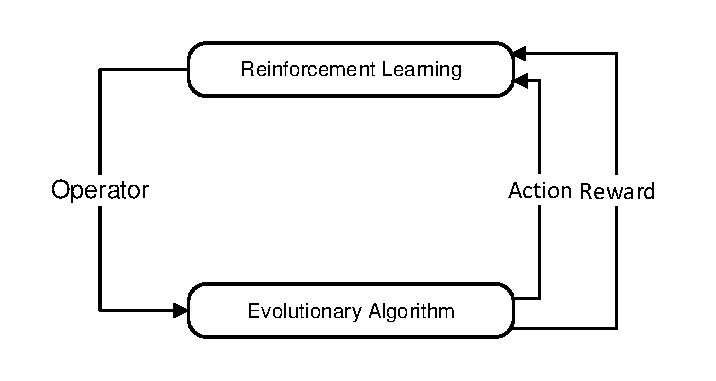
\includegraphics[width=0.8\linewidth]{figs/RLEA1.pdf}}
  \caption{Interaction framework between RL and EA}
  \label{fig:RLEA}
\end{figure}
% 强化学习主要由agent environment state action reward 组成,agent根据环境的状态执行某个动作,之后环境会转换到一个新的状态,并且根据新的状态环境会给出奖励信号,agent根据奖励调整策略,agent的目标是得到最大的累积奖励。
RL is composed of agent, environment, state, action and reward, the agent takes action according to the state of the environment, and then the environment will change to a new state and give a reward value, the agent will adjust its strategy according to the reward and agent's goal is to get the maximum cumulative reward.

%%% 再说明如何建模成MDP使得RL应用到AOS问题
% 可以看到AOS和强化学习面临相同的问题,1. 根据当前的状态做出决策,并得到反馈。2. 根据反馈调整策略
AOS and RL face the same issues:
\begin{enumerate}
  \item Make decisions based on the current state and get feedback.
  \item Adjust the strategy according to the feedback.
\end{enumerate}
%%% 将AOS建模成MDP问题。
% 基于这些相似的问题,我们可以利用RL做AOS,
Based on these similar issues, we can use RL to solve AOS problems.
% 首先需要将进化过程建模为MDP,具有如下定义
First, we model the evolution procedure as an MDP,
% MDP是agent与environment交互,以最大化累计reward的数学模型, 在AOS问题中,agent作为controller,负责选择算子,并根据应用算子后的反馈调整选择策略。environment是整个进化算法框架,本文使用MOEA/D框架,负责利用agent给出的算子生成子代,并计算子代的适应度值,向agent返回reward。
MDP is a mathematical model in which an agent interacts with the environment to maximize cumulative reward, in AOS problems the agent as a controller, is responsible for selecting the operator and adjusting the selection strategy according to the feedback after the operator is applied.
Environment is the whole framework of evolutionary algorithm, this paper uses the MOEA/D framework, which is responsible for using the operator given by agent to generate the offspring, calculating the fitness value of the offspring, and returning the reward to agent.
% 为了应用MDP,我们还需要给出状态、动作、奖励的定义
To apply the MDP, we also need to give the definition of state, action and reward.
\begin{enumerate}
  \item \textit{State:}
        % 状态是对当前环境的描述,也是agent做出决策的依据,我们把父代的决策变量x_i, 分解向量w_i作为状态S_i
        The state is the description of the current environment and the basis for the agent to make decisions. We take the decision variable $x$ of the parent, decomposition vector $W$ as the state $s_t$.
        \begin{equation}
          s_{t}=\left\{x_{1,t}^i, x_{2,t}^i, \ldots, x_{D,t}^i, W_{1}^{i}, \ldots, W_{m}^{i}\right\}
        \end{equation}
        % x是t时刻第i个个体的D维决策变量,w是第i个个体的权重向量。
        % 由于不同的个体有不同的最佳算子,因此父代的决策变量是必须的。在MOEA/D框架下,多目标被分解成多个单目标,不同的权重组合构成不同的目标,因此分解向量对最佳算子的选择也有影响。
        Since different individuals have different optimal operators, the decision variables are necessary. In the framework of MOEA/D, multi-objective are decomposed into a set of single-objective, and different weight combinations constitute different objectives, so the decomposition vector also has an impact on the selection of the best operator.
  \item \textit{Action:}
        % 在MDP中,agent根据环境的状态做出动作,具体来说,深度神经网络输出在当前状态下每个动作质量,之后使用operator selection的方法给出具体的算子。
        In MDP, the agent makes an action $a_t$ based on the state $s^i$, specifically, the deep neural network outputs the quality of each action in the current state, and then uses the operator selection \ref{operator_selection} method to give the recommended operator.
        % \TODO{action space}
        % 动作空间是
        % \TODO{add equation}
        % \item \textit{Policy:}
  \item \textit{Reward:}
        % 执行动作a^i后,状态会从S^i转移到S^i+1,并且环境会通过比较两个状态给出reward,表示动作的好坏。奖励越大,说明算子的效果越好,通过调整策略,在下次类似的状态时有更大的概率应用相同的算子。
        State will be transferred from $s_{t}$ to $s_{t+1}$ with action $a_t$, and the environment will give a reward $r_{t+1}$ by comparing the two states, indicating the quality of the action $a_t$. A larger reward indicates that the operator has a better performance, by adjusting strategy, the agent is more likely to apply the same operator in the next similar state.
        % \TODO{add equation}
\end{enumerate}

%%% 说明用的MOEA/D框架
% 由于在多目标中很难量化子代和父代的性能差异,因此大多数AOS methods被设计应用到单目标问题上。
Most AOS methods were designed for single-objective problems because it is difficult to measure the performance difference between an offspring and a parent.
% 比如基于支配的多目标算法 NSGAII,SPEA2,大多数解都是非支配的。
For example, in domination relation based multi-objective algorithms, such as NSGA-II \cite{nsga2} and SPEA2 \cite{spea2}, most of the solutions are non-dominated, so it is difficult to determine the fitness improvement rate.
% 我们使用MOEAD算法,which可以将多目标问题分解成多个单目标子问题,所以单目标中适应度赋值的方法可以应用moead框架上。
In this paper, MOEA/D is applied, which can decompose MOP into several single-objective subproblems, so the methods of credit assignment in single-objective can be applied to the MOEA/D framework.

%%% 应用的是DQN的强化学习方法
% 由于算子选择问题具有离散的动作空间,因此我们使用RL的variant,DQN 
Since the AOS problems have discrete action space, a variant of the RL, deep Q learning (DQN) is applied.
% 将MOEA/D框架作为环境,与DQN交互。
The MOEA/D framework is used as the environment to interacts with DQN,
% MOEA/D-DQN的伪代码
the details of MOEA/D-DQN are shown in Algorithm \ref{alg:moead-dqn}.

\begin{algorithm}[t]
  \label{alg:moead-dqn}
  \caption{Framework of MOEA/D-DQN}
  \SetKwComment{Comment}{//}{}
  \small
  % \KwIn{}
  % \KwOut{}
  % 初始化各种参数
  $\mathcal{P} = \{x^i,\dots,x^N\}$: The initial population\;
  $\lambda = \{\lambda^i,\dots,\lambda^N\}$: The weight vectors\;
  $z^* = \{z_1,\dots,z_m\}^T$: The best value found so far objective $f_i$\;
  $\mathcal{D}$: Experience replay pool\;
  $N_D$: The experience replay pool maximum size\;
  $N_b$: Training batch size\;
  $Q$: The primary action-value network\;
  $\hat{Q}$: The target action-value network\;
  % $\gamma$: The discount factor\;
  % $C$: The 

  % while 评价次数t<FE^max
  \While{ the termination critera have not been met}{
  The indexes of the subproblems whose objectives are MOP individual objectives $f_i$ are selected to form initial $I$ and add other $\frac{N}{5} - m$ indexes to $I$ by using 10-tournament selection based on $\pi^i$.
  % 索引 i in (1,,NP)
  \ForEach{$i \in I$}{
  \If{$rand(0,1) < \delta$}{
    $P = B(i)$\;
  }\Else{
    $P = \mathcal{P}$\;
  }
  $op = Operator Selection(x^i, \lambda^i)$\;
  Generate the offspring $y$ by applying the chosen operator $op$ and the polynomial mutation operator\;
  Update the best value $z^*$ if $z_j > f_j(y)$\;
  $reward = Credit Assignment(op, y)$\;
  %%%%% 根据reward更新DQN权重
  Store the transition $(s_t, a_t, r_{t+1}, s_{t+1})$ in replay buffer $\mathcal{D}$,
  replacing the oldest transition if $|\mathcal{D}| >= N_D$\;
  Sample a batch of $N_b$ transitions $(s_j,a_j,r_{j+1},s_{j+1})$ from $\mathcal{D}$\;
  $y_j = r_j + \gamma \max{_{a^\prime} \hat{Q}(s_{j+1}, a^\prime)}$\;
  Calculate the loss $\mathcal{L} = \frac{1}{N_b} \sum_{i=1}^{N_b}(Q(s_j,a_j)-y_j)^2$\;
  Update $Q$ using the SGD algorithm by minimizing the loss $\mathcal{L}$\;
  Every $C$ steps, copy the weight of $Q$ to $\hat{Q}$\;
  }
  % 更新pi
  $gen$++\;
  \If {$mod(gen,50)=0$}{
    update the utility $\pi^i$ of each subproblem\;
  }
  }
  % transtion = (s_t, a_t, r_t, u_i)
  % 利用DQN 使用 transtion更新网络

\end{algorithm}

% 在时刻t,个体的决策变量和权重向量共同组成state s,作为神经网络的输入,神经网络的输出是一个n维向量 out,表示应用算子后可以得到的期望累计回报,根据输出向量基于轮盘赌选择一个算子op,应用算子产生子代off,在基于分解的多目标框架中,我们可以很容易的计算子代相对于父代的适应度值提高率FIR,将应用的算子和得到的FIR放入滑动窗口中,之后从滑动窗口中取出算子op对应的最大FIR作为reward r,使用DQN算法更新RL的策略以最大化累积奖励。
At the time $t$, state $s_t$ is composed of individual decision variables and weight vector as the input of the neural network. The output of the neural network is an n-dim vector $\text{out}_t$, which represents the expected cumulative reward after the application of the operator.
According to the $\text{out}_t$, an operator $op_i$ is selected based on roulette, and the $op_t$ is used to generate the offspring $\text{off}_t$. In the multi-objective framework based on decomposition, we can easily calculate the $\text{FIR}_t$, put the $op_i$ and $\text{FIR}_t$ into the sliding window, then take the maximum FIR corresponding to the operator $op_i$ from the sliding window as the reward $r_t$, then use the DQN algorithm to update the RL strategy to maximize the cumulative reward.



\section{Experimental studies}
%%% 实验研究
% 为了证明算法MOEA/D-DQN的有效性,我们在 xxx 数据集进行了测试,并且和MOEA/D-DE,MOEA/D-DRA,MOEA/D-FRRMAB,MOEA/D-IR比较了结果。
%  \TODO 增加参考文献引用
To prove the effectiveness of MOEA/D-DQN, we test it on ZDT, DTLZ, WFG , UF datasets, and compare the results with those obtained by MOEA/D-DE, MOEA/D-DRA, MOEA/D-FRRMAB, MOEA/D-IR.

\subsection{Experimental settings}
% 对比算法的参数设置参考原论文的实现,结果来自PlatEMO platform
All the parameters in the comparison algorithm are the same as those in the original paper, and the experimental results are collected from PlatEMO \cite{PlatEMO} platform.
% 算法的参数设置如下
The parameters of our method MOEA/D-DQN are set as follows.
\begin{enumerate}
  \item Parameters in operators: $CR=1$, $F=0.5$, $K=0.5$, $\eta=20$;
  \item Population size $N$ is set 100 for ZDT, DTLZ and WFG, 600/1000 for bi/tri-objective UF;
  \item Maximum number of solutions replaced by each offspring $n_r$ is 2;
  \item The neighborhood size: $T=20$;
  \item Control parameters in operators: We set the $F=0.5$ and $CR=1.0$ for DE operators, and the distribution index $\eta=20$ in SBX.
  \item Control parameters in MOEA/D-DQN:
        \begin{enumerate}
          \item The length of window \textit{windowSize} equal to population size $N$;
          \item The train batch size: $N_b = 16$;
          \item The experience replay pool maximum size: $N_D=512$;
        \end{enumerate}
\end{enumerate}

%%%% 算法跑30次,评价次数
% 对于每个test instances, 算法独立运行30次,
All test instances run on the same computer(Intel$\circledR$ $\text{Core}^{\text{TM}}$ i7-8700K CPU @ 3.70GHz, 32 GB), for each test instance, all algorithms run 30 times independently, in order to ensure the fairness of the comparison, all algorithms use the same number of function evaluations,
the algorithm stops running when the number of evaluations is reached.
% 评价次数设置
We set the number of function evaluations for the ZDT test instances as 10,000, the DTLZ test instances as 30,000, the WFG test instances as 25,000, and the UF test instances as 300,000.
% 秩和检验,显著性分析
To obtain a statistically comprehensive conclusion, we conducted the Wilcoxon rank sum test between the data obtained by the comparison algorithms, and the significant difference was 0.05.
% "+-="
"+" ,"-" ,"=" denote the results of the compared algorithms are better than, worse than, and similar to those obtained by proposed MOEA/D-DQN.

%%%%% 评价指标
No single performance metric can give a comprehensive measure of the performance of an MOEA, in this paper, we chose two widely used performance indicators: Inverted generational distance (IGD) \cite{igd} and Hypervolume (HV) \cite{hv}.
% igd
Both of them can measure the convergence and distribution of the population, in order to calculate the IGD, we uniformly sample 10,000 points from the real PF of each problem to constitute a reference set. The smaller the IGD value, the closer the solutions are to the real PF.
% HV
We set $y^* = (y^*_1, \dots, y^*_m)$ as a point in the objective space which is dominated by any Pareto vectors. Let $S$ be the obtained non-dominated solutions in the objective space. Then the $I_{HV}$ value of $S$ is the volume of the region weakly dominated by $S$ and $y^*$. The larger of the Hypervolume, the better of the approximation. In our experiments, we set $y^* = (1,\dots, 1).$

\subsection{Experimental results}
%%%%%%% 比较MOEA/D-DQN和对比算法在所有测试问题上的IGD和HV
% 我们测试了MOEA/D-DQN和4个对比算法在ZDT和UF测试实例上的效果,IGD值are shown in Table 1,
We compared MOEA/D-DQN and four comparison algorithms on ZDT, DTLZ, WFG and UF test instances, Table \ref{tab:igd_all} Table \ref{tab:hv_all} show the mean and standard deviation of IGD and HV in 30 independent runs.

% 可以看到在大多数问题上,MOEA/D-DQN都获得了最好的效果。
From the tables \ref{tab:igd_all} and \ref{tab:hv_all}, we can see that the MOEA/D-DQN has achieved the best results in most problems, and the results of IGD and HV indicators are consistent. In total, among the five comparison algorithms, it has obtained the best results in 19 out of 31 performance for IGD and 20 out of 31 for HV.




\begin{table*}[tbp]
  \renewcommand{\arraystretch}{1.2}  % 行间距
  \centering
  \caption{IGD values obtained by MOEA/D-FRRMAB, MOEA/D-DYTS, MOEA/D-DRA, MOEA/D-M2M and proposed MOEA/D-DQN on ZDT, DTLZ, WFG and UF, where the best result in each row is highlighted.}
  \begin{tabular}{cccccc}
    \toprule
    Problem & MOEA/D-FRRMAB              & MOEA/D-DYTS                & MOEA/D-DRA                 & MOEA/D-M2M                 & MOEA/D-DQN               \\
    \midrule
    ZDT1    & 3.8123e-2 (2.14e-2) -      & 3.8144e-2 (2.08e-2) -      & 1.9377e-1 (5.73e-2) -      & 1.0701e-1 (8.16e-2) -      & \hl{6.9980e-3 (1.76e-3)} \\
    ZDT2    & 1.2262e-1 (5.89e-2) -      & 1.1662e-1 (4.88e-2) -      & 3.0430e-1 (1.14e-1) -      & 8.3664e-2 (8.14e-2) -      & \hl{2.4188e-2 (2.15e-2)} \\
    ZDT3    & 1.9540e-1 (4.85e-2) -      & 2.0511e-1 (4.72e-2) -      & 3.1938e-1 (5.43e-2) -      & 2.4879e-1 (8.09e-2) -      & \hl{1.7122e-2 (5.58e-3)} \\
    ZDT4    & 7.8472e+0 (4.44e+0) -      & 3.9875e+0 (3.34e+0) -      & 1.1806e+1 (6.89e+0) -      & 1.7537e+1 (5.17e+0) -      & \hl{2.5453e-1 (9.70e-2)} \\
    ZDT6    & 4.2009e-3 (3.96e-3) =      & \hl{3.5353e-3 (9.44e-4) =} & 5.3427e-2 (1.06e-1) -      & 6.6665e-3 (5.75e-4) -      & 3.8825e-3 (2.74e-3)      \\
    \hline
    DTLZ1   & 3.4192e-1 (6.12e-1) -      & 6.3591e-1 (9.08e-1) -      & 1.2916e+0 (1.53e+0) -      & 1.8884e+0 (1.30e+0) -      & \hl{1.8507e-2 (8.58e-4)} \\
    DTLZ2   & 7.5370e-2 (6.65e-4) -      & 7.5319e-2 (5.90e-4) -      & 7.5716e-2 (6.94e-4) -      & 1.5040e-1 (5.57e-3) -      & \hl{4.7007e-2 (1.53e-4)} \\
    DTLZ3   & 1.8153e+1 (1.89e+1) -      & 1.7439e+1 (2.28e+1) -      & 2.5743e+1 (2.40e+1) -      & 4.2691e+1 (1.86e+1) -      & \hl{1.2903e+0 (3.04e+0)} \\
    DTLZ4   & 1.2233e-1 (7.09e-2) -      & 1.6551e-1 (9.04e-2) -      & 2.2549e-1 (1.76e-1) -      & 1.0034e-1 (5.65e-3) -      & \hl{4.7086e-2 (2.36e-4)} \\
    DTLZ5   & 1.4252e-2 (1.58e-4) +      & 1.4401e-2 (1.19e-4) +      & \hl{1.4166e-2 (1.45e-4) +} & 3.8102e-2 (5.07e-3) -      & 2.6538e-2 (5.78e-4)      \\
    DTLZ6   & 1.4528e-2 (5.14e-5) +      & 1.4537e-2 (3.79e-5) +      & \hl{1.4338e-2 (6.68e-5) +} & 3.0851e-2 (4.53e-3) =      & 2.9008e-2 (4.72e-5)      \\
    DTLZ7   & 1.9837e-1 (3.99e-2) -      & 2.1575e-1 (7.33e-2) -      & 2.2761e-1 (6.01e-2) -      & 6.7829e-1 (1.82e-1) -      & \hl{1.1006e-1 (3.56e-4)} \\
    \hline
    WFG1    & 1.5443e+0 (7.38e-2) -      & 1.4408e+0 (1.09e-1) -      & 1.3536e+0 (8.07e-2) -      & 1.3838e+0 (6.52e-2) -      & \hl{7.1675e-1 (8.33e-2)} \\
    WFG2    & 3.6394e-1 (3.00e-2) -      & 3.5163e-1 (2.96e-2) -      & 3.4125e-1 (2.29e-2) -      & 2.8906e-1 (1.05e-2) -      & \hl{2.0742e-1 (1.96e-2)} \\
    WFG3    & 2.1493e-1 (3.59e-2) -      & 1.9109e-1 (4.03e-2) -      & 1.8917e-1 (3.15e-2) -      & 3.1880e-1 (3.19e-2) -      & \hl{1.2825e-1 (4.77e-3)} \\
    WFG4    & 3.9968e-1 (1.25e-2) -      & 3.9868e-1 (1.57e-2) -      & 3.8005e-1 (1.12e-2) -      & 3.5696e-1 (1.34e-2) -      & \hl{2.3703e-1 (5.38e-3)} \\
    WFG5    & 3.3880e-1 (4.34e-3) -      & 3.3789e-1 (5.03e-3) -      & 3.3639e-1 (4.02e-3) -      & 3.4891e-1 (1.60e-2) -      & \hl{2.2353e-1 (3.01e-3)} \\
    WFG6    & 4.3816e-1 (3.03e-2) -      & 4.3740e-1 (4.00e-2) =      & 4.3393e-1 (2.83e-2) =      & 4.8888e-1 (1.54e-2) -      & \hl{4.2542e-1 (4.02e-2)} \\
    WFG7    & 3.6693e-1 (9.62e-3) =      & \hl{3.6391e-1 (7.96e-3) =} & 3.6897e-1 (1.03e-2) =      & 3.9817e-1 (1.79e-2) -      & 3.6882e-1 (1.13e-2)      \\
    WFG8    & \hl{4.4389e-1 (2.41e-2) +} & 4.5188e-1 (4.59e-2) +      & 4.7517e-1 (4.77e-2) =      & 4.9053e-1 (2.17e-2) =      & 4.8352e-1 (5.64e-2)      \\
    WFG9    & 3.8344e-1 (4.80e-2) =      & 3.4880e-1 (3.77e-2) +      & \hl{3.4008e-1 (1.98e-2) =} & 3.4430e-1 (1.70e-2) =      & 3.5458e-1 (3.56e-2)      \\
    \hline
    UF1     & 2.3837e-3 (1.94e-3) =      & 2.7501e-2 (7.77e-2) =      & 1.9429e-3 (7.06e-4) -      & 1.4966e-2 (5.03e-3) -      & \hl{1.3666e-3 (1.05e-4)} \\
    UF2     & 3.0706e-3 (9.33e-4) -      & 2.0981e-3 (7.41e-4) =      & 3.8904e-3 (1.98e-3) -      & 6.2214e-3 (4.85e-4) -      & \hl{2.0228e-3 (4.02e-4)} \\
    UF3     & \hl{1.8076e-2 (1.59e-2) =} & 2.5324e-2 (2.19e-2) =      & 2.7810e-2 (4.57e-2) =      & 1.9927e-2 (6.68e-3) =      & 2.1607e-2 (1.97e-2)      \\
    UF4     & 5.1265e-2 (2.86e-3) -      & 4.9417e-2 (2.48e-3) -      & 6.1483e-2 (4.47e-3) -      & 4.3390e-2 (7.10e-4) -      & \hl{3.3923e-2 (1.36e-3)} \\
    UF5     & 5.2543e-1 (1.38e-1) =      & 6.3341e-1 (1.26e-1) -      & 5.3079e-1 (1.07e-1) =      & \hl{3.0405e-1 (5.98e-2) +} & 5.2563e-1 (1.62e-1)      \\
    UF6     & 4.4067e-1 (6.41e-2) -      & 4.5274e-1 (4.32e-2) -      & 3.9160e-1 (7.58e-2) =      & \hl{1.3534e-1 (2.27e-2) +} & 3.7661e-1 (7.47e-2)      \\
    UF7     & 2.2646e-1 (2.61e-1) -      & 3.1521e-1 (2.59e-1) -      & 2.3092e-1 (2.48e-1) -      & \hl{8.9138e-3 (2.41e-3) +} & 3.1031e-2 (1.06e-1)      \\
    UF8     & \hl{9.6619e-2 (2.88e-2) +} & 1.0052e-1 (1.29e-2) +      & 1.1058e-1 (5.11e-2) +      & 1.0220e-1 (2.16e-2) +      & 1.2196e-1 (7.22e-2)      \\
    UF9     & 1.6370e-1 (5.13e-2) =      & 1.8932e-1 (6.28e-3) -      & 1.7194e-1 (3.57e-2) -      & 1.3742e-1 (4.25e-2) =      & \hl{1.2445e-1 (6.56e-2)} \\
    UF10    & 8.5939e-1 (1.29e-1) -      & 6.6767e-1 (8.06e-2) -      & \hl{4.7879e-1 (7.97e-2) +} & 1.0107e+0 (1.40e-1) -      & 5.3962e-1 (1.80e-1)      \\
    \hline
    +/-/=   & 4/20/7                     & 5/20/6                     & 4/20/7                     & 4/22/5                     &                          \\
    \bottomrule
  \end{tabular}
  \label{tab:igd_all}
\end{table*}

\begin{table*}[tbp]
  \renewcommand{\arraystretch}{1.2}  % 行间距
  \centering
  \caption{HV values obtained by MOEA/D-FRRMAB, MOEA/D-DYTS, MOEA/D-DRA, MOEA/D-M2M and proposed MOEA/D-DQN on ZDT, DTLZ, WFG and UF, where the best result in each row is highlighted.}
  \begin{tabular}{cccccc}
    \toprule
    Problem & MOEA/D-FRRMAB              & MOEA/D-DYTS                & MOEA/D-DRA                 & MOEA/D-M2M                 & MOEA/D-DQN               \\
    \midrule
    ZDT1    & 6.5008e-1 (4.21e-2) -      & 6.5144e-1 (3.94e-2) -      & 4.3095e-1 (6.07e-2) -      & 5.8492e-1 (1.02e-1) -      & \hl{7.1383e-1 (3.22e-3)} \\
    ZDT2    & 3.4137e-1 (4.81e-2) -      & 3.3871e-1 (4.17e-2) -      & 1.8242e-1 (8.59e-2) -      & 3.4648e-1 (8.72e-2) -      & \hl{4.2482e-1 (1.97e-2)} \\
    ZDT3    & 4.0050e-1 (4.99e-2) -      & 3.9482e-1 (4.97e-2) -      & 2.9291e-1 (4.11e-2) -      & 4.5588e-1 (6.27e-2) -      & \hl{5.7176e-1 (6.68e-3)} \\
    ZDT4    & 0.0000e+0 (0.00e+0) -      & 1.8324e-2 (5.51e-2) -      & 0.0000e+0 (0.00e+0) -      & 0.0000e+0 (0.00e+0) -      & \hl{3.6640e-1 (9.68e-2)} \\
    ZDT6    & 3.8756e-1 (3.81e-3) =      & \hl{3.8820e-1 (7.74e-4) =} & 3.5118e-1 (6.31e-2) -      & 3.8370e-1 (9.72e-4) -      & 3.8782e-1 (3.12e-3)      \\
    \hline
    DTLZ1   & 4.5973e-1 (3.37e-1) -      & 2.9816e-1 (3.45e-1) -      & 1.5896e-1 (2.78e-1) -      & 3.0600e-2 (1.14e-1) -      & \hl{8.4290e-1 (2.60e-3)} \\
    DTLZ2   & 5.2680e-1 (2.02e-3) -      & 5.2742e-1 (1.46e-3) -      & 5.2744e-1 (1.75e-3) -      & 3.6835e-1 (1.22e-2) -      & \hl{5.6260e-1 (1.08e-3)} \\
    DTLZ3   & 1.0455e-1 (1.89e-1) -      & 7.3842e-2 (1.55e-1) -      & 2.9014e-2 (1.12e-1) -      & 0.0000e+0 (0.00e+0) -      & \hl{2.2500e-1 (2.18e-1)} \\
    DTLZ4   & 5.1875e-1 (2.30e-2) -      & 5.0512e-1 (2.90e-2) -      & 4.7030e-1 (8.27e-2) -      & 4.7119e-1 (1.13e-2) -      & \hl{5.6242e-1 (1.55e-3)} \\
    DTLZ5   & 1.9439e-1 (1.04e-4) +      & \hl{1.9447e-1 (6.85e-5) +} & 1.9437e-1 (1.32e-4) +      & 1.6757e-1 (5.95e-3) -      & 1.8605e-1 (3.54e-4)      \\
    DTLZ6   & 1.9474e-1 (1.71e-5) +      & 1.9474e-1 (1.25e-5) +      & \hl{1.9484e-1 (2.91e-5) +} & 1.8193e-1 (2.74e-3) -      & 1.8459e-1 (3.71e-5)      \\
    DTLZ7   & 2.0189e-1 (2.78e-2) -      & 1.9794e-1 (2.67e-2) -      & 1.7790e-1 (3.21e-2) -      & 4.5193e-2 (3.74e-2) -      & \hl{2.6054e-1 (9.41e-4)} \\
    \hline
    WFG1    & 2.6850e-1 (3.21e-2) -      & 3.3736e-1 (4.74e-2) -      & 3.4552e-1 (2.76e-2) -      & 3.5987e-1 (1.95e-2) -      & \hl{5.9691e-1 (4.54e-2)} \\
    WFG2    & 8.8930e-1 (7.11e-3) -      & 8.8887e-1 (5.60e-3) -      & 8.8943e-1 (7.79e-3) -      & 8.7498e-1 (6.41e-3) -      & \hl{9.0955e-1 (4.47e-3)} \\
    WFG3    & 3.2653e-1 (2.14e-2) -      & 3.3520e-1 (2.85e-2) -      & 3.4071e-1 (2.01e-2) -      & 2.9131e-1 (1.75e-2) -      & \hl{3.7149e-1 (2.69e-3)} \\
    WFG4    & 4.6426e-1 (6.46e-3) -      & 4.6709e-1 (7.48e-3) -      & 4.6253e-1 (6.91e-3) -      & 4.7668e-1 (7.88e-3) -      & \hl{5.1279e-1 (5.51e-3)} \\
    WFG5    & 4.5819e-1 (2.97e-3) -      & 4.5693e-1 (3.23e-3) -      & 4.5844e-1 (3.04e-3) -      & 4.7358e-1 (6.16e-3) -      & \hl{4.9979e-1 (1.88e-3)} \\
    WFG6    & 3.8792e-1 (4.59e-2) -      & 3.9318e-1 (4.92e-2) =      & 3.9247e-1 (4.02e-2) =      & 3.6610e-1 (1.18e-2) -      & \hl{4.0557e-1 (4.59e-2)} \\
    WFG7    & \hl{4.9630e-1 (6.18e-3) =} & 4.9598e-1 (5.46e-3) =      & 4.9527e-1 (6.49e-3) =      & 4.7953e-1 (6.71e-3) -      & 4.9322e-1 (6.75e-3)      \\
    WFG8    & 3.8395e-1 (1.77e-2) +      & \hl{4.0356e-1 (3.14e-2) +} & 3.6446e-1 (3.13e-2) =      & 3.7039e-1 (1.07e-2) =      & 3.6046e-1 (3.70e-2)      \\
    WFG9    & 4.1859e-1 (6.21e-2) =      & 4.6132e-1 (4.63e-2) =      & 4.7170e-1 (2.41e-2) =      & \hl{4.9096e-1 (7.05e-3) +} & 4.5656e-1 (4.38e-2)      \\
    \hline
    UF1     & 7.2001e-1 (3.98e-3) -      & 6.8333e-1 (1.15e-1) =      & 7.2111e-1 (1.38e-3) -      & 7.0455e-1 (6.88e-3) -      & \hl{7.2239e-1 (1.56e-4)} \\
    UF2     & 7.2011e-1 (1.18e-3) -      & 7.2127e-1 (9.52e-4) =      & 7.1921e-1 (2.56e-3) -      & 7.1664e-1 (7.09e-4) -      & \hl{7.2149e-1 (7.63e-4)} \\
    UF3     & 6.8973e-1 (2.88e-2) =      & 6.7574e-1 (3.78e-2) =      & 6.7501e-1 (7.48e-2) =      & \hl{6.9709e-1 (8.10e-3) =} & 6.8253e-1 (3.44e-2)      \\
    UF4     & 3.7669e-1 (3.93e-3) -      & 3.7652e-1 (4.09e-3) -      & 3.5933e-1 (5.62e-3) -      & 3.8955e-1 (1.08e-3) -      & \hl{4.0228e-1 (1.70e-3)} \\
    UF5     & 1.0720e-1 (4.80e-2) -      & 1.0232e-1 (4.34e-2) -      & 1.6883e-1 (7.02e-2) =      & \hl{1.6980e-1 (5.50e-2) =} & 1.6464e-1 (8.54e-2)      \\
    UF6     & 1.1748e-1 (5.96e-2) =      & 8.5356e-2 (9.96e-3) -      & 1.8770e-1 (7.70e-2) =      & \hl{3.3665e-1 (2.34e-2) +} & 1.5061e-1 (7.33e-2)      \\
    UF7     & 3.9157e-1 (2.04e-1) -      & 3.0724e-1 (2.17e-1) -      & 3.9266e-1 (2.02e-1) -      & \hl{5.7320e-1 (3.54e-3) +} & 5.5683e-1 (9.68e-2)      \\
    UF8     & 4.7737e-1 (2.57e-2) +      & \hl{4.8312e-1 (3.45e-3) +} & 4.7104e-1 (4.43e-2) +      & 4.3191e-1 (1.88e-2) +      & 4.2908e-1 (5.75e-2)      \\
    UF9     & 6.6877e-1 (3.70e-2) =      & 6.4829e-1 (8.11e-3) -      & 6.7034e-1 (3.06e-2) =      & 6.6850e-1 (3.63e-2) =      & \hl{6.7685e-1 (5.89e-2)} \\
    UF10    & 7.3765e-3 (1.80e-2) -      & 4.7815e-2 (2.86e-2) -      & 1.3150e-1 (6.41e-2) =      & 6.4038e-4 (3.37e-3) -      & \hl{1.5583e-1 (7.11e-2)} \\
    \hline
    +/-/=   & 4/21/6                     & 4/20/7                     & 3/19/9                     & 4/23/4                     &                          \\
    \bottomrule
  \end{tabular}
  \label{tab:hv_all}
\end{table*}

%%%% 排名
To see the overall performances, Table \ref{tab:rank_all} shows the average ranking of IGD and HV on all 31 test instances.
% 可以看出前4个算法差别不大,而MOEA/D-DQN明显优于其它算法
It can be seen that the first four algorithms have little difference, and MOEA/D-DQN is better than other algorithms, the results of different indicators are consistent.


\begin{table*}[tbp]
  \renewcommand{\arraystretch}{1.2}  % 行间距
  \centering
  \caption{The average ranks of the compared algorithms according to their IGD and HV on the 31 test instances.}
  \begin{tabular}{cccccc}
    \toprule
    Alg. & MOEA/D-FRRMAB & MOEA/D-DYTS & MOEA/D-DRA & MOEA/D-M2M & MOEA/D-DQN \\
    \midrule
    IGD  & 3.0323        & 3.1613      & 3.3871     & 3.5806     & 1.8387     \\
    HV   & 3.0645        & 3.1290      & 3.3226     & 3.4516     & 1.9032     \\
    \bottomrule
  \end{tabular}
  \label{tab:rank_all}
\end{table*}

%%%%%% 和单个算子的对比,可能比不过,但排名或许能比得过
% 通常来说,没有一个算子可以在所有问题上都有好的效果,为了研究不同算子在不同问题上的表现,我们比较了单个算子和.. 为了保证公平,除了算子外,其他部分与MOEA/D-DQN一致,
Generally speaking, no operator can achieve good results on all problems, in order to study the performance of different operators on different problems, MOEA/D-DQN is compared with four MOEA/D variants, each of them using only one operator from the operator pool to produce offspring. The other parts of the comparison algorithms are consistent with MOEA/D-DQN except for the operator.

% 表格展示了单个了单个算子和MOEA/D-DQN在31个测试问题上的IGD值和HV值,以及算法在每个测试问题上的排名
Tables \ref{tab:igd_ops}, \ref{tab:hv_ops} present the IGD and HV values of five algorithms on 31 test instances, as well as the ranks of the algorithms on each instance and the overall ranks of the according to their average rank values on all instances.
% 从表中可以看出,
From tables \ref{tab:igd_ops}, \ref{tab:hv_ops}, we can see that each operator has distinct performance on different instances. In general, our algorithm has the best performance, ranking second on average and top 3 on most instances.

\begin{table*}[tbp]
  \renewcommand{\arraystretch}{1.2}  % 行间距
  \centering
  \caption{IGD values obtained by MOEA/D-DQN and MOEA/D with single operator on ZDT, DTLZ, WFG and UF over 30 runs and the ranks}
  \begin{tabular}{cccccc}
    \toprule
    Problem         & MOEA/D-OP1 (rank)   & MOEA/D-OP2 (rank)   & MOEA/D-OP3 (rank) & MOEA/D-OP4 (rank)   & MOEA/D-DQN (rank)   \\
    \midrule
    ZDT1            & 1.1554e-02 (2)      & 3.6240e-02 (3)      & 4.4362e-02 (4)    & 5.2718e-02 (5)      & \hl{6.9980e-03 (1)} \\
    ZDT2            & \hl{2.0159e-02 (1)} & 6.0830e-02 (3)      & 1.0700e-01 (4)    & 1.4857e-01 (5)      & 2.4188e-02 (2)      \\
    ZDT3            & 4.3307e-02 (2)      & 2.2010e-01 (4)      & 2.2983e-01 (5)    & 2.0123e-01 (3)      & \hl{1.7122e-02 (1)} \\
    ZDT4            & \hl{1.2382e-01 (1)} & 6.2584e-01 (3)      & 1.2818e+00 (4)    & 1.7178e+01 (5)      & 2.5453e-01 (2)      \\
    ZDT6            & 4.5689e-02 (5)      & \hl{3.1665e-03 (1)} & 1.0660e-02 (4)    & 9.2326e-03 (3)      & 3.8825e-03 (2)      \\
    \hline
    DTLZ1           & 3.0622e-02 (2)      & 3.9651e-01 (3)      & 7.6483e-01 (4)    & 1.4942e+00 (5)      & \hl{1.8507e-02 (1)} \\
    DTLZ2           & 7.5314e-02 (5)      & 7.4957e-02 (2)      & 7.5180e-02 (3)    & 7.5271e-02 (4)      & \hl{4.7007e-02 (1)} \\
    DTLZ3           & \hl{2.7189e-01 (1)} & 1.1206e+01 (3)      & 2.3510e+01 (5)    & 1.9302e+01 (4)      & 1.2903e+00 (2)      \\
    DTLZ4           & 4.8295e-01 (5)      & 1.2165e-01 (2)      & 2.2932e-01 (4)    & 1.4300e-01 (3)      & \hl{4.7086e-02 (1)} \\
    DTLZ5           & 1.4594e-02 (4)      & 1.4395e-02 (3)      & 1.4333e-02 (2)    & \hl{1.4327e-02 (1)} & 2.6538e-02 (5)      \\
    DTLZ6           & 1.4605e-02 (4)      & 1.4565e-02 (3)      & 1.4521e-02 (2)    & \hl{1.4517e-02 (1)} & 2.9008e-02 (5)      \\
    DTLZ7           & 2.1389e-01 (5)      & 1.9859e-01 (2)      & 2.0422e-01 (4)    & 1.9953e-01 (3)      & \hl{1.1006e-01 (1)} \\
    \hline
    WFG1            & \hl{3.1491e-01 (1)} & 7.2333e-01 (3)      & 1.3045e+00 (4)    & 1.5719e+00 (5)      & 7.1675e-01 (2)      \\
    WFG2            & 3.2499e-01 (3)      & 3.1654e-01 (2)      & 3.4742e-01 (4)    & 3.6405e-01 (5)      & \hl{2.0742e-01 (1)} \\
    WFG3            & \hl{1.1023e-01 (1)} & 1.9606e-01 (4)      & 1.9143e-01 (3)    & 2.1869e-01 (5)      & 1.2825e-01 (2)      \\
    WFG4            & 3.6323e-01 (2)      & 3.9103e-01 (4)      & 3.9770e-01 (5)    & 3.8302e-01 (3)      & \hl{2.3703e-01 (1)} \\
    WFG5            & 3.5804e-01 (4)      & 3.5895e-01 (5)      & 3.4197e-01 (3)    & 3.3582e-01 (2)      & \hl{2.2353e-01 (1)} \\
    WFG6            & \hl{3.7771e-01 (1)} & 4.3557e-01 (5)      & 4.1647e-01 (3)    & 4.1171e-01 (2)      & 4.2542e-01 (4)      \\
    WFG7            & \hl{3.5699e-01 (1)} & 3.7839e-01 (5)      & 3.6778e-01 (3)    & 3.6413e-01 (2)      & 3.6882e-01 (4)      \\
    WFG8            & \hl{4.1146e-01 (1)} & 5.2766e-01 (5)      & 4.6258e-01 (3)    & 4.4173e-01 (2)      & 4.8352e-01 (4)      \\
    WFG9            & 3.7346e-01 (4)      & 3.9139e-01 (5)      & 3.5906e-01 (3)    & \hl{3.4276e-01 (1)} & 3.5458e-01 (2)      \\
    \hline
    UF1             & 1.3930e-01 (5)      & 1.4971e-02 (3)      & 2.9363e-02 (4)    & 1.7860e-03 (2)      & \hl{1.3666e-03 (1)} \\
    UF2             & 1.7842e-02 (5)      & 2.5884e-03 (2)      & 2.6555e-03 (3)    & 2.8186e-03 (4)      & \hl{2.0228e-03 (1)} \\
    UF3             & 3.4550e-01 (5)      & 1.5582e-01 (4)      & 8.3464e-02 (3)    & \hl{1.6469e-02 (1)} & 2.1607e-02 (2)      \\
    UF4             & 4.8002e-02 (2)      & 5.4258e-02 (5)      & 5.3660e-02 (4)    & 5.2840e-02 (3)      & \hl{3.3923e-02 (1)} \\
    UF5             & 5.1969e-01 (3)      & 5.0021e-01 (2)      & 5.3475e-01 (5)    & \hl{4.7151e-01 (1)} & 5.2563e-01 (4)      \\
    UF6             & 4.3553e-01 (4)      & 4.1098e-01 (3)      & 4.0028e-01 (2)    & 4.3869e-01 (5)      & \hl{3.7661e-01 (1)} \\
    UF7             & 5.3382e-01 (5)      & 2.3914e-01 (3)      & 3.8103e-01 (4)    & 1.7435e-01 (2)      & \hl{3.1031e-02 (1)} \\
    UF8             & 2.1644e-01 (5)      & 1.8533e-01 (4)      & 1.1518e-01 (2)    & \hl{8.5514e-02 (1)} & 1.2196e-01 (3)      \\
    UF9             & 1.7807e-01 (4)      & 2.1211e-01 (5)      & 1.6876e-01 (3)    & \hl{1.3883e-01 (1)} & 1.5445e-01 (2)      \\
    UF10            & \hl{4.4170e-01 (1)} & 5.2621e-01 (2)      & 6.5396e-01 (4)    & 1.0753e+00 (5)      & 5.3962e-01 (3)      \\
    \hline
    rank statistics & 3.0322581 (2)       & 3.3225806 (4)       & 3.5483871 (5)     & 3.0322581 (2)       & \hl{2.0645161 (1)}  \\
    \bottomrule
    \label{tab:igd_ops}
  \end{tabular}
\end{table*}

% HV
\begin{table*}[tbp]
  \renewcommand{\arraystretch}{1.2}  % 行间距
  \centering
  \caption{HV values obtained by MOEA/D-DQN and MOEA/D-DRA with single operator on ZDT, DTLZ, WFG and UF over 30 runs and the ranks}
  \begin{tabular}{cccccc}
    \toprule
    Problem         & MOeA/D-OP1 (rank)   & MOeA/D-OP2 (rank)   & MOeA/D-OP3 (rank) & MOeA/D-OP4 (rank)   & MOeA/D-DQN (rank)   \\
    \midrule
    ZDT1            & 7.0742e-01 (2)      & 6.5708e-01 (3)      & 6.3983e-01 (4)    & 6.2583e-01 (5)      & \hl{7.1383e-01 (1)} \\
    ZDT2            & \hl{4.2606e-01 (1)} & 3.9024e-01 (3)      & 3.5377e-01 (4)    & 3.1372e-01 (5)      & 4.2482e-01 (2)      \\
    ZDT3            & 5.6112e-01 (2)      & 3.7786e-01 (4)      & 3.6753e-01 (5)    & 3.9834e-01 (3)      & \hl{5.7176e-01 (1)} \\
    ZDT4            & \hl{5.3410e-01 (1)} & 1.3076e-01 (3)      & 9.1378e-02 (4)    & 0.0000e+00 (5)      & 3.6640e-01 (2)      \\
    ZDT6            & 3.5829e-01 (5)      & \hl{3.8833e-01 (1)} & 3.8234e-01 (3)    & 3.8215e-01 (4)      & 3.8782e-01 (2)      \\
    \hline
    DTLZ1           & 8.0439e-01 (2)      & 4.7802e-01 (3)      & 3.5536e-01 (4)    & 1.4404e-01 (5)      & \hl{8.4290e-01 (1)} \\
    DTLZ2           & 5.2850e-01 (2)      & 5.2587e-01 (4)      & 5.2715e-01 (3)    & 5.2392e-01 (5)      & \hl{5.6260e-01 (1)} \\
    DTLZ3           & \hl{3.9864e-01 (1)} & 6.3222e-02 (4)      & 6.6517e-02 (3)    & 3.4538e-02 (5)      & 2.2500e-01 (2)      \\
    DTLZ4           & 3.4554e-01 (5)      & 5.1975e-01 (2)      & 4.7145e-01 (4)    & 5.1261e-01 (3)      & \hl{5.6242e-01 (1)} \\
    DTLZ5           & \hl{1.9470e-01 (1)} & 1.9449e-01 (3)      & 1.9452e-01 (2)    & 1.9415e-01 (4)      & 1.8605e-01 (5)      \\
    DTLZ6           & 1.9471e-01 (4)      & 1.9472e-01 (3)      & 1.9475e-01 (2)    & \hl{1.9476e-01 (1)} & 1.8459e-01 (5)      \\
    DTLZ7           & 2.3352e-01 (2)      & 2.2809e-01 (3)      & 2.0545e-01 (4)    & 1.8258e-01 (5)      & \hl{2.6054e-01 (1)} \\
    \hline
    WFG1            & \hl{9.0433e-01 (1)} & 7.3401e-01 (2)      & 3.9703e-01 (4)    & 2.4776e-01 (5)      & 5.9691e-01 (3)      \\
    WFG2            & 8.7480e-01 (5)      & 8.8278e-01 (4)      & 8.8844e-01 (2)    & 8.8690e-01 (3)      & \hl{9.0955e-01 (1)} \\
    WFG3            & \hl{3.7880e-01 (1)} & 3.2560e-01 (5)      & 3.3607e-01 (3)    & 3.2673e-01 (4)      & 3.7149e-01 (2)      \\
    WFG4            & \hl{5.1565e-01 (1)} & 4.9819e-01 (3)      & 4.7183e-01 (4)    & 4.5914e-01 (5)      & 5.1279e-01 (2)      \\
    WFG5            & 4.7010e-01 (3)      & 4.7052e-01 (2)      & 4.6062e-01 (4)    & 4.5732e-01 (5)      & \hl{4.9979e-01 (1)} \\
    WFG6            & \hl{4.5676e-01 (1)} & 3.9750e-01 (5)      & 4.1894e-01 (3)    & 4.2413e-01 (2)      & 4.0557e-01 (4)      \\
    WFG7            & \hl{5.1595e-01 (1)} & 5.0229e-01 (2)      & 4.9977e-01 (3)    & 4.9302e-01 (5)      & 4.9322e-01 (4)      \\
    WFG8            & \hl{4.3187e-01 (1)} & 3.6014e-01 (5)      & 3.7638e-01 (3)    & 3.8037e-01 (2)      & 3.6046e-01 (4)      \\
    WFG9            & 4.6367e-01 (2)      & 4.4771e-01 (5)      & 4.5096e-01 (4)    & \hl{4.6722e-01 (1)} & 4.5656e-01 (3)      \\
    \hline
    UF1             & 5.3534e-01 (5)      & 6.9251e-01 (3)      & 6.7636e-01 (4)    & 7.2134e-01 (2)      & \hl{7.2239e-01 (1)} \\
    UF2             & 7.0612e-01 (5)      & 7.2041e-01 (3)      & 7.2025e-01 (4)    & 7.2053e-01 (2)      & \hl{7.2149e-01 (1)} \\
    UF3             & 3.0682e-01 (5)      & 4.8089e-01 (4)      & 5.8544e-01 (3)    & \hl{6.9277e-01 (1)} & 6.8253e-01 (2)      \\
    UF4             & 3.8530e-01 (2)      & 3.7258e-01 (4)      & 3.7166e-01 (5)    & 3.7413e-01 (3)      & \hl{4.0228e-01 (1)} \\
    UF5             & 1.5003e-01 (3)      & 1.6368e-01 (2)      & 1.2867e-01 (4)    & 9.9957e-02 (5)      & \hl{1.6464e-01 (1)} \\
    UF6             & 1.5683e-01 (2)      & \hl{1.7700e-01 (1)} & 1.3239e-01 (4)    & 1.2928e-01 (5)      & 1.5061e-01 (3)      \\
    UF7             & 1.9419e-01 (5)      & 3.8387e-01 (3)      & 2.6289e-01 (4)    & 4.4318e-01 (2)      & \hl{5.5683e-01 (1)} \\
    UF8             & 3.9928e-01 (5)      & 4.2579e-01 (4)      & 4.7403e-01 (2)    & \hl{4.8215e-01 (1)} & 4.2908e-01 (3)      \\
    UF9             & 6.4602e-01 (4)      & 6.3983e-01 (5)      & 6.6986e-01 (3)    & \hl{6.8912e-01 (1)} & 6.7685e-01 (2)      \\
    UF10            & \hl{1.7226e-01 (1)} & 1.0879e-01 (3)      & 4.9183e-02 (4)    & 7.9704e-04 (5)      & 1.5583e-01 (2)      \\
    \hline
    rank statistics & 2.6129032 (5)       & 3.2580645 (2)       & 3.5161290 (3)     & 3.5161290 (3)       & \hl{2.0967742 (1)}  \\
    \bottomrule
    \label{tab:hv_ops}
  \end{tabular}
\end{table*}

%%%% 算子应用比例
% 我们已经证明了基于DQN的算子选择方法比应用单个算子有更好的效果,但我们仍不知道算子选择只是选择最佳的单个算子,亦或是在不同阶段有不同的算子处于支配地位。为了研究算子的应用轨迹,我们调查了在搜索过程中每个算子应用比例的变化。
We have proved that the operator selection based on DQN has a better effect than a single operator, but we still do not understand that operator selection is only to select the best single operator, or there are different operators in different states. In order to study the application trajectories of operators, we investigate the change of the application proportion of each operator in the search process.
% 为了使得不同阶段区别更加明显,我们每隔10代统计一次算子的应用数量,并在图中画出了算子在整个进化阶段的应用比例,
In order to make the distinction between different stages more obvious, we count the number of operators applied every 10 generations and draw the proportion of operators applied in the whole evolution stage in Fig. \ref{fig:tra}.

% 从图可以我们看出,在任何测试实例上,没有一个操作员能够主宰整个搜索过程。在开始阶段,由于RL的探索特性,算子选择的策略类似于随机选择, 之后的每个阶段都有单个算子处于支配地位,在不同搜索阶段,支配算子会逐渐从一个算子切换为另一个。
As we can see from Fig. \ref{fig:tra}, no operator can dominate the whole search process on any of the test instances. In the initial stage, due to the exploration characteristics of RL, the mechanism of operator selection is similar to random selection, after which a single operator is dominant at each stage, and the dominant operator gradually switches from one operator to another at different search stages.


\begin{figure*}[t]
  \centering
  \subfloat[Operator selection trajectory on UF2.]{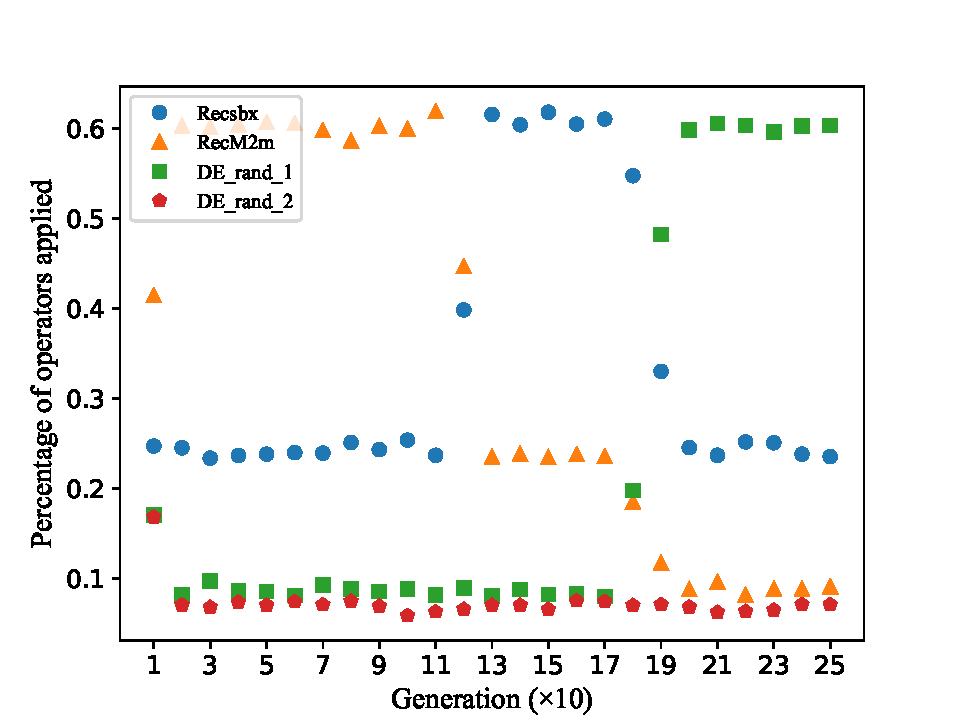
\includegraphics[width=0.33\linewidth]{figs/ops_uf2.pdf}}\hfil
  \subfloat[Operator selection trajectory on UF6.]{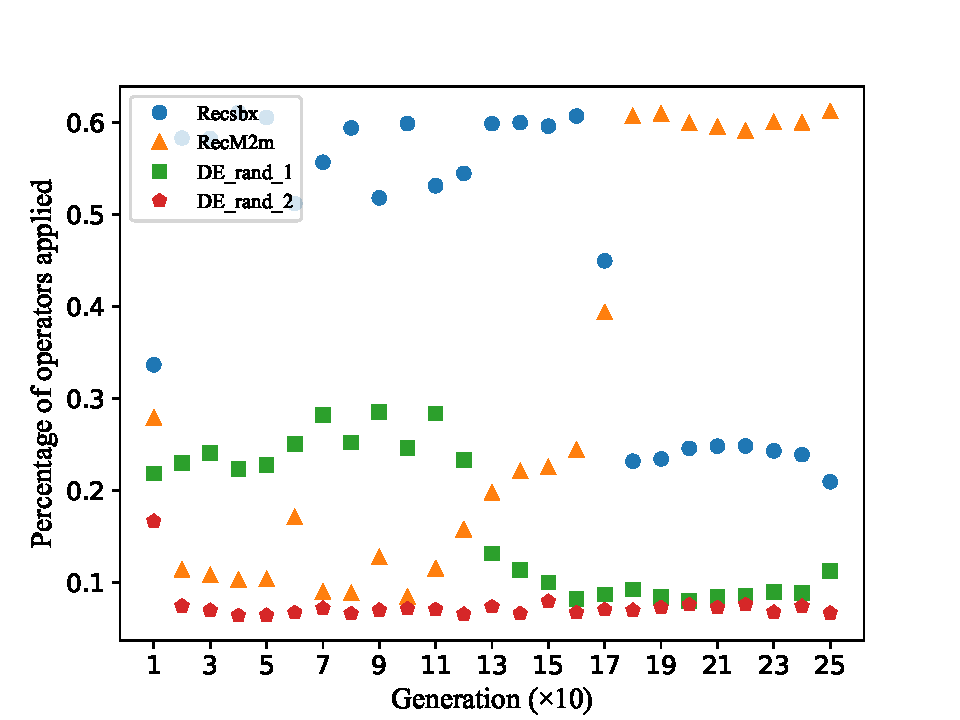
\includegraphics[width=0.33\linewidth]{figs/ops_uf6.pdf}}\hfil
  \subfloat[Operator selection trajectory on UF7.]{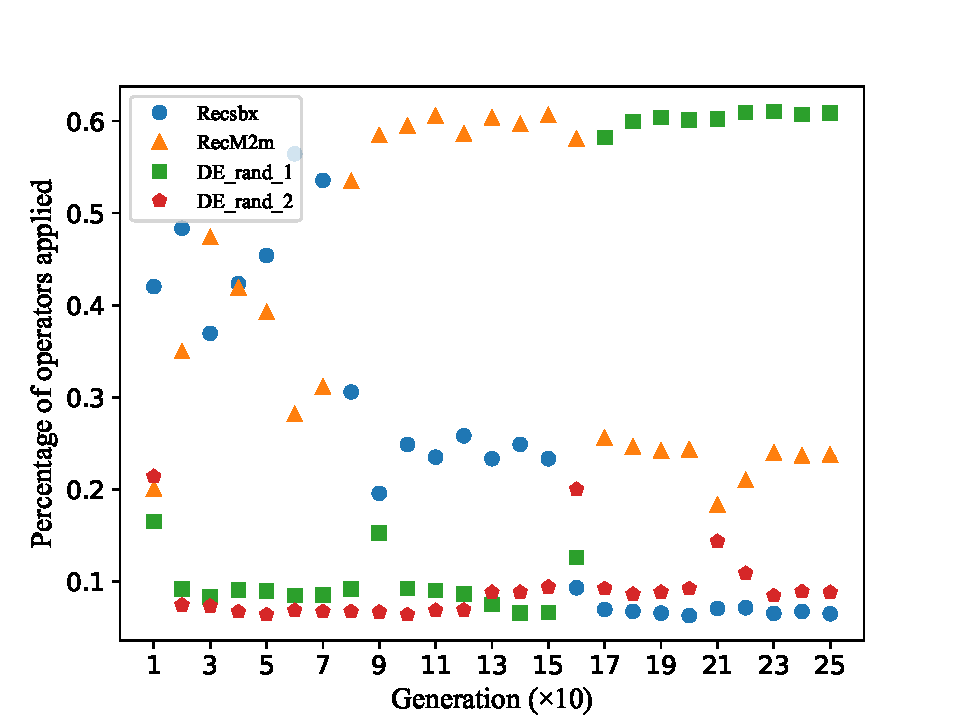
\includegraphics[width=0.33\linewidth]{figs/ops_uf7.pdf}}\hfil
  \subfloat[Operator selection trajectory on UF8.]{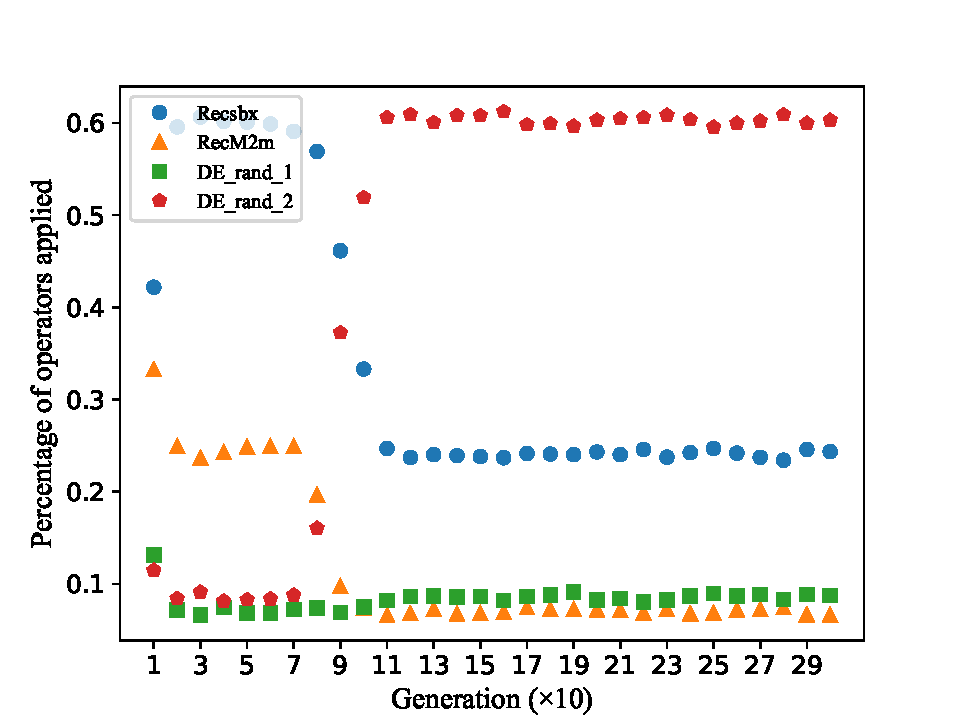
\includegraphics[width=0.33\linewidth]{figs/ops_uf8.pdf}}\hfil
  \subfloat[Operator selection trajectory on UF9.]{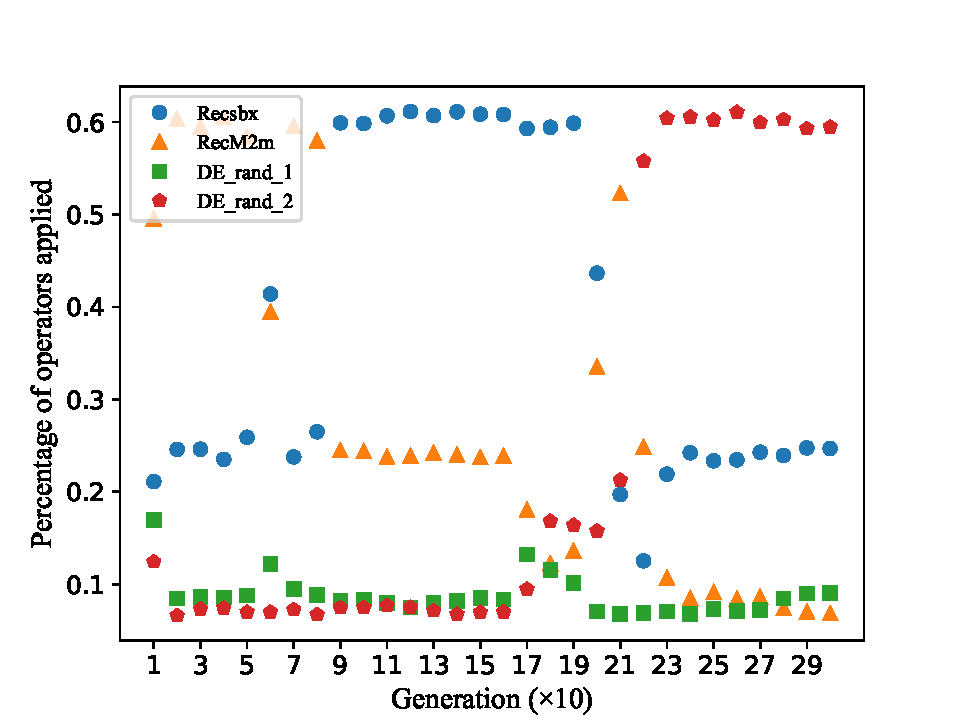
\includegraphics[width=0.33\linewidth]{figs/ops_uf9.pdf}}\hfil
  \subfloat[Operator selection trajectory on UF10.]{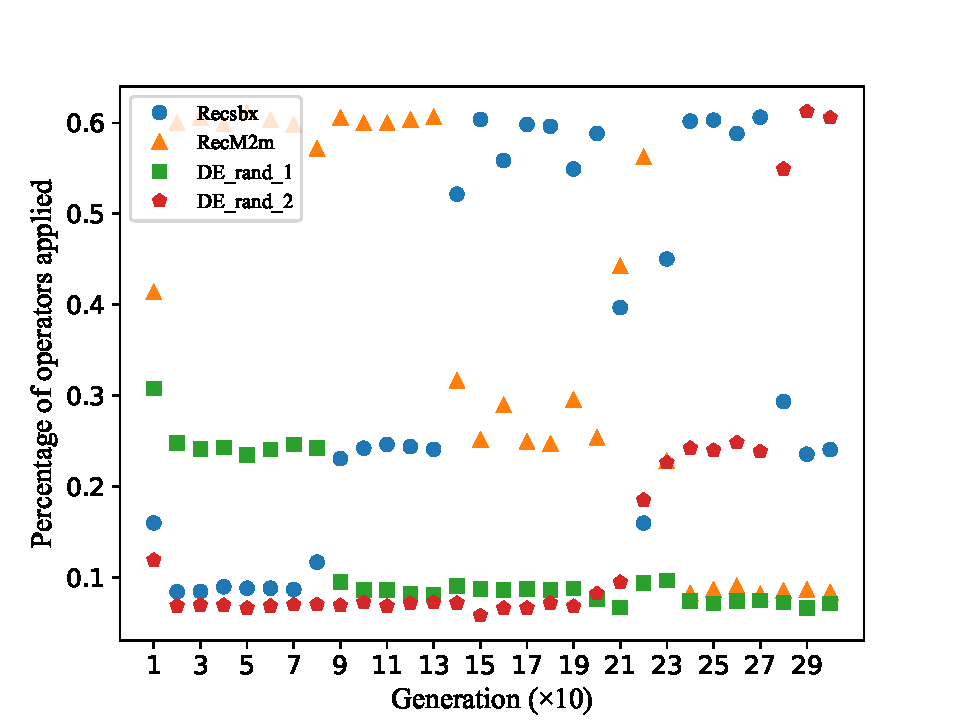
\includegraphics[width=0.33\linewidth]{figs/ops_uf10.pdf}}\\
  \caption{Operator selection trajectories of MOEA/D-DQN}
  \label{fig:tra}
\end{figure*}

%%%%% IGD值的下降,或许降得更快


\section{Conclusions}
In this paper, an adaptive operator selection based on a Deep Q network (MOEA/D-DQN) is proposed.
% 建模成MDP,使用深度神经网络作为算子选择器,同时也是强化学习的策略。
The adaptive operator selection problem was modeled MDP, we use the deep neural network as an operator selector, which is also a reinforcement learning strategy.
% 我们将适应度提高率作为RL的reward,适应度提高率由生成的子代和被替换的父代个体决定
We take the fitness improvement rate as the RL's reward, and the FIR is determined by the generated offspring and the replaced parent.
% ,由于进化过程的不稳定性,我们设计了一个固定长度的队列用来store the FIR values of the recently used operators, 为了更好的表示算子的效果,我们取队列中的最大值FIR作为算子的reward反馈给RL
Due to the instability of the evolutionary process, we design a fixed-length queue to store the FIR values of the recently used operators, and to better represent the effect of the operator, we take the maximum value of FIR of the corresponding operator in the queue as the reward feedback to RL.
% MOEA/D-DQN通过在线控制的方法,一边对环境采样,一边通过采样得到的数据学习,节省了训练时间,而且比起预训练的方法, MOEA/D-DQN在新的问题上有更好的表现。
MOEA/D-DQN can save the training time by online control and learning from the sampled data. Moreover, compared with the pre-training method, MOEA/D-DQN has better performance on new problems.
% 实验结果表明,该算法具有较强的竞争力,说明了该控制器的有效性。
The experimental results showed that the AOS based on RL was very competitive to the compared algorithms, which shows the effectiveness of the proposed controller.

% 图x显示不同的算子适用于不同的问题,并且在同一个问题的不同阶段,最佳算子也是不同的。这说明算子选择不光能够减少人工设计参数的复杂性,而且对提升算法的性能是有必要的。
Fig. \ref{fig:tra} shows that different operators are suitable for different problems and that the optimal operator is different in different stages of the same problem, this shows that operator selection not only reduces the complexity of manually designed parameters but is also necessary to improve the performance of the algorithm.
This is well illustrated by the results in Table \ref{tab:igd_ops} and Table \ref{tab:hv_ops}.

% 之后的工作, 我们希望设计更有效的state来充分说明当前种群的信息,MOEA/D-DQN中的state只和当前个体有关,而忽略了种群中不同个体之间的联系,并且仅以当前个体的fitness improvement作为reward有可能导致陷入局部最优,虽然基于群体智能的进化算法在一定程度上可以避免局部最优,但维护种群的多样性也是有必要的,因此在之后的工作中,我们计划在state和reward同时考虑种群的收敛性和分布性的,根据种群的状态确定当前应该偏向探索或是利用。
In the future, we hope to design a more effective state to represent the information of the current population, the state in MOEA/D-DQN is only determined by the current individual but ignores the connection between different individuals in the population, and only using fitness improvement as the reward may lead to local optimization, although the evolutionary algorithm can avoid local optimization to a certain extent, it is necessary to maintain the diversity of the population. Therefore, in the future work, we plan to represent both the convergence and distribution of the population in the state and reward of RL and to determine exploration or exploitation depend on the state of the population.
% 除了用RL做算子选择,自适应参数控制也是一个很重要的领域,基于policy optimazation的RL方法可以生成实数范围的连续动作作为算法的参数,更进一步,我们可以使用生成式的模型,直接生成子代,避免使用固定生成算子的局限
In addition to using RL as operator selection, adaptive parameter control is also a very important field. RL based on policy optimization can generate continuous actions as the parameters of operators. Furthermore, we can use a generative model to generate offspring directly, avoiding the limitation of using fixed operators.


\ifCLASSOPTIONcaptionsoff
  \newpage
\fi

\bibliographystyle{IEEEtran}
\bibliography{references}



\end{document}